\chapter{BULGULAR VE İRDELEME \label{sec:YapilanCalismalar}}

Tez çalışmasında önerilen yaklaşımlar, pankreas hastalıkları bulunan kişilerin sağkalım oranını artırmak, tanı, tedavi ve cerrahide tıp doktorlarına yardımcı olmak için pankreas ve pankreas tümörü segmentasyonu gerçekleştirmektedirler. Tez çalışmasının bu bölümünde ilk olarak önerilen yaklaşımların gerçekleştirildiği cihaz konfigürasyonu hakkında bilgiler verilecektir. Daha sonra çalışma kapsamında önerilen yaklaşımların abdominal kontrastlı pankreas BT dilimleri üzerinde gerçekleştirilen deneyleri, elde edilen görsel ve sayısal sonuçları irdelenecektir. Gerçekleştirilen tez çalışması pankreas ve pankreas tümörü segmentasyonu olmak üzere iki kısımdan oluşmaktadır. Bu iki kısım için elde edilen bulgular ve önerilen yaklaşımların literatürdeki çalışmalarla kıyaslanmaları ilgili ana başlıklar altında ayrı ayrı verilecektir.
 
Tez çalışmasında birinci kısım olan Pankreas Segmentasyonu için NIH veri seti, ikinci kısım olan Pankreas ve Pankreas Tümörü Segmentasyonu için MSD veri seti kullanılmaktadır. Çalışmada önerilen yaklaşımların analizi için kullanılan veri setlerinin ayrıntılı açıklamaları Bölüm \ref{sec:genel}’de ilgili alt başlıklar altında verilmektedir. Dolayısıyla bu bölümde tekrar veri seti analizi yapılmayacaktır. 

\section{Cihaz Konfigürasyonu}
Pankreas segmentasyonunun gerçekleştirildiği tez çalışmasının ilk kısmını Pankreas İlgi Bölgesinin Belirlenmesi ve Belirlenen İlgi Bölgesinde Pankreas Segmentasyonu fazları oluşturmaktadır. Pankreas ve pankreas tümörü segmentasyonunun gerçekleştirildiği ikinci kısım ise Pankreas İlgi Bölgesinin Belirlenmesi, Belirlenen İlgi Bölgesinde Pankreas ve Pankreas Tümörü Segmentasyonu fazlarından oluşmaktadır. 

Tez çalışmasının ilk kısmı Intel Core i7-9750 2.60 GHz işlemci, 32 GB RAM ve NVIDIA GeForce RTX 2060 GPU 6GB VRAM 1920 CUDA çekirdeği bulunan bir bilgisayarda çalışan Pyton 3.6 yazılımı ile arka planda Tensorflow kütüphanesini kullanan Keras kütüphanesi temelli bir cihaz yapılandırması kurularak gerçekleştirilmiştir. Bu kısımda kaynak tüketimi az yüksek doğruluklu pakreas segmentasyonu gerçekleştiren bir yöntem önerilmiştir.

Tez çalışmasının ikinci kısmı AMD Ryzen 7 3800x 3.90 GHz işlemci, 32 GB RAM ve NVIDIA GeForce RTX 3060 GPU 12GBVRAM 3584 CUDA çekirdeği bulunan bir bilgisayarda çalışan Pyton 3.6 yazılımı ile arka planda Tensorflow kütüphanesini kullanan Keras kütüphanesi temelli bir cihaz yapılandırması kurularak gerçekleştirilmiştir. Bu kısımda ilk kısımda önerilen yöntem pankreas ve pankreas tümör segmentasyonu gerçekleştirebilmek amacı ile tekrar ele alınmış ve farklı derin öğrenme teknikleri ile zenginleştirilmiştir.

\section{Pankreas İlgi Bölgesinin Belirlenmesi ve İlgi Bölgesinde Pankreas Segmentasyonu ile Elde Edilen Deneysel Sonuçlar}

\subsection{Önerilen Ağ Mimarilerinin Özellikleri}
Pankreas Segmentasyonu için önerilen iki aşamalı yöntemin ilk fazı olan Pankreas İlgi Bölgesinin Belirlenmesi'nde Waleed Abdulla tarafından geliştirilen Keras ve Tensorflow tabanlı Mask R-CNN modeli \cite{he2017mask} ResNet-101 çekirdek ağı ile kullanılmaktadır. Bu model orijinal olarak renkli görüntülerin segmentasyonu için kullanılmaktadır. Ancak yapılan çalışmada giriş katmanı gri seviyedeki biyomedikal görüntüleri alacak şekilde yapılandırılmaktadır. Bu modelde eğitim sürecindeki dinamik öğrenme katsayısı, doğrulama kaybı değerine göre güncellenmektedir.

Pankreas Segmentasyonu için önerilen iki aşamalı yöntemin ikinci fazı olan Pankreas Segmentasyonu’nda, önceki fazda (Pankreas İlgi Bölgesinin Belirlenmesi) elde edilen alt BT dilimlerinde pankreas bölgelerini belirlemek için 3B U-Net modeli kullanılmaktadır. Bu modelin geliştirilmesi için orijinal 2B U-Net'ten ilham alınmaktadır \cite{ronneberger2015u}. Bu modelin giriş katmanları, 3B alt BT dilimlerinden bütün veri alacak şekilde yapılandırılmaktadır. Ek olarak, bu modeldeki tüm katmanlar (3B Konvolüsyon, 3B Maksimum Havuzlama, vb.), 3B hacimsel girişi işlemek için yeniden tasarlanmaktadır.

Pankreas Segmentasyonu için önerilen iki aşamalı yöntemdeki Pankreas İlgi Bölgesinin Belirlenmesi ve Pankreas Segmentasyonu fazlarının eğitim ve test süreçleri için standart çapraz doğrulama stratejisi kullanılmaktadır. NIH veri setinin (82 hasta) rastgele bölünmesinde dört kat (fold) çapraz doğrulama gerçekleştirilmektedir. Tasarlanan Mask R-CNN ve 3B U-Net modellerinde eğitim iterasyonları her kat için 100.000'de durdurulmaktadır. Otomatik pankreas segmentasyonu için tasarlanan Pankreas İlgi Bölgesinin Belirlenmesi (Mask R-CNN) ve Pankreas Segmentasyonu (3B U-Net) fazlarının eğitim süreleri sırasıyla yaklaşık 7 ve 1 gün sürmektedir. Pankreas İlgi Bölgesinin Belirlenmesi (Mask R-CNN) ve Pankreas Segmentasyonu (3B U-Net) fazlarının test süreçlerinde ise bir BT dilimi için ortalama çalışma süresi yaklaşık 20 saniye olarak hesaplanmaktadır.

\subsection{Pankreas İlgi Bölgesinin Belirlenmesi ve İlgi Bölgesinde Pankreas Segmentasyonu ile Elde Edilen Sayısal Sonuçlar}

Bu tez çalışmasında radyolog tarafından manuel olarak işaretlenmiş pankreas bölgeleri ile önerilen CNN tabanlı yöntemler kullanılarak segmente edilmiş pankreas bölgeleri arasındaki benzerliğini göstermek için ROC eğrisi kullanılmaktadır. Şekil \ref{fig:roc-curve-auc}’de NIH veri setinde önerilen yaklaşım ile elde edilen 1, 2, 3 ve 4 katlarının ROC eğrilerini sunulmaktadır. Her kat için elde edilen değerler sırasıyla \%99.29, \%99.21, \%99.08 ve \%99.17’dir. NIH veri setinde önerilen yaklaşım ile elde edilen ortalama ROC eğrisi değeri \%99.19 iken standart sapma değeri 0.08 olarak hesaplanmaktadır. Şekil \ref{fig:roc-curve-auc}’de gösterilen ROC eğrisi sonuçlarına göre radyolog tarafından manuel olarak işaretlenmiş pankreas bölgeleri ile önerilen CNN tabanlı yaklaşımlar ile segmente edilmiş pankreas bölgeleri arasındaki benzerlik oldukça yüksektir.

\captionsetup[figure]{margin={0.4cm,-2.7cm}}
\begin{figure}[h!]
	\begin{center}
		\vspace{0.4cm}
		\captionbox{NIH veri setinde önerilen yaklaşım ile elde edilen 1, 2, 3 ve 4 katlarının ROC eğrileri. \label{fig:roc-curve-auc}}
		{
			\vspace{0.4cm}
			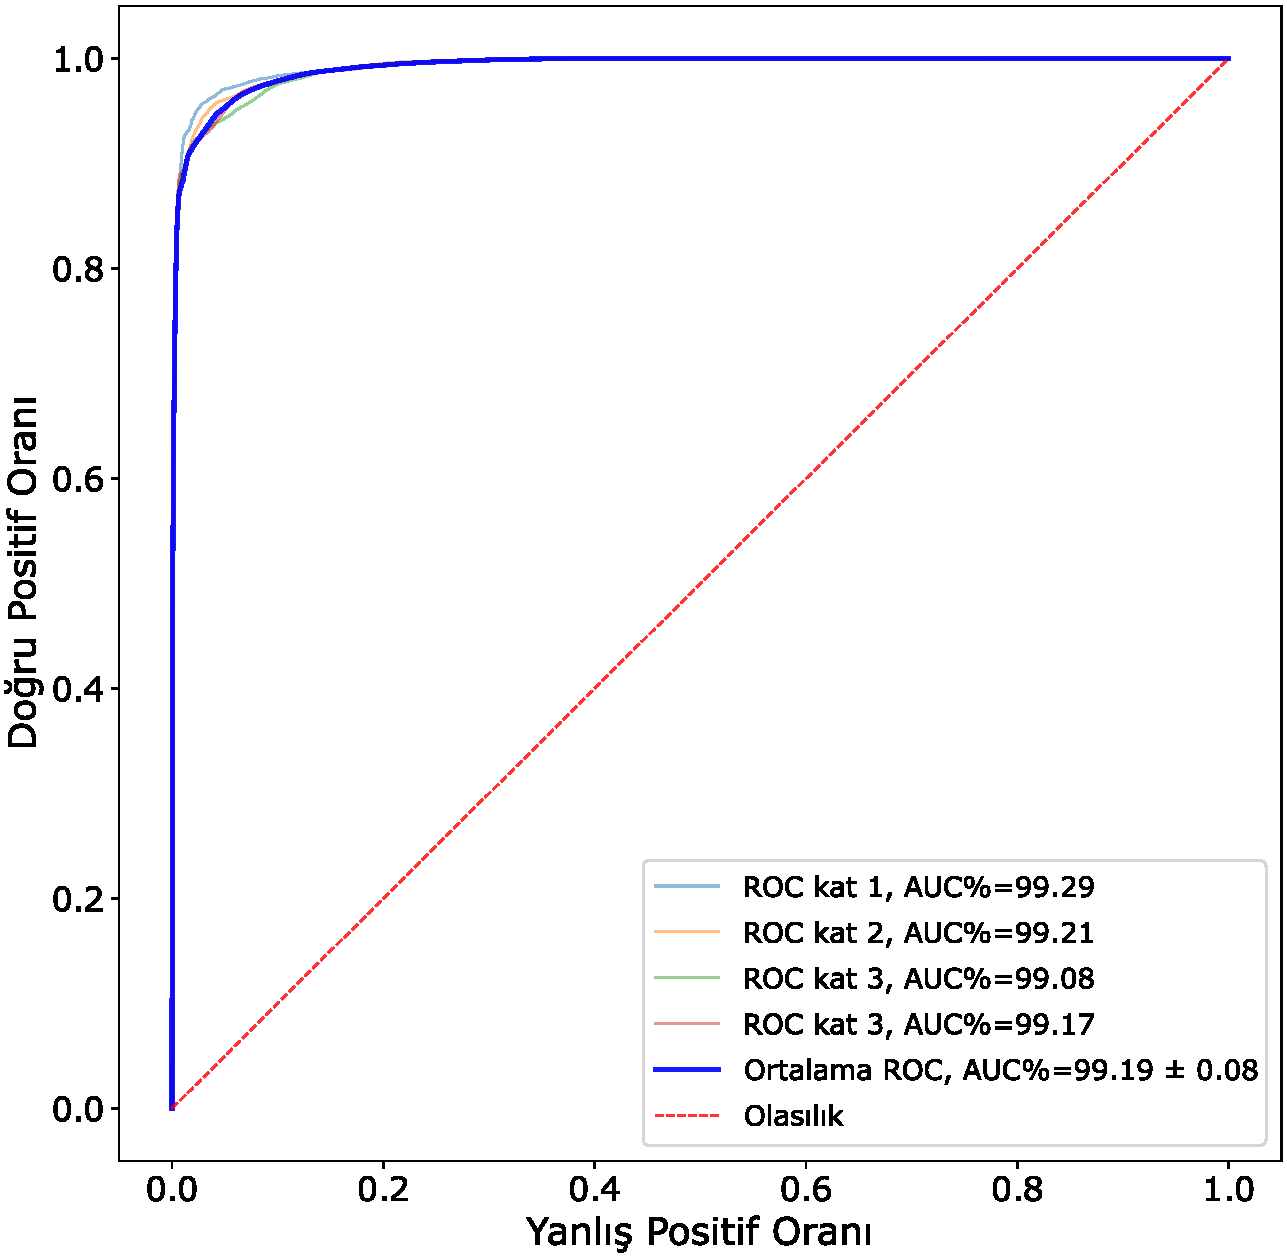
\includegraphics[scale=0.45]{Bulgular-Irdeleme/Figures/roc-curve-auc.pdf}
		}
	\end{center}
\end{figure}

\begin{sidewaystable}[htpb]
	\centering
	\caption{Pankreas Segmentasyonu için sadece birinci fazın (Pankreas İlgi Bölgesinin Belirlenmesi - Mask R-CNN) kullanılması durumunda performans değerlendirme metriklerinin sonuçları (Ortalama$\pm$STD[MIN,MAK])}
	\label{tab:mrcnn_result}
	\begin{adjustbox}{width=\textwidth}		
		\begin{tabular}{cccccccc}
			\toprule
			Kat   &  DSC \%       &  JI  \%   &  PRE  \%   &  REC  \%  & ACC  \%  &  SPE  \% &  AUC  \% \\ 
			\midrule 
			1       & 80.94$\pm$4.02[69.81,84.41] & 68.16$\pm$5.42[53.62,73.03] & 81.33$\pm$5.39[70.14,91.99] & 80.84$\pm$5.26[69.49,87.90] & 99.94$\pm$0.02[99.90,99.96]  & 99.97$\pm$0.01[99.95,99.99]  &  - \\
			2       & 81.48$\pm$4.14[69.31,85.66] & 68.94$\pm$5.59[53.03,74.92] & 82.37$\pm$4.77[68.53,89.87] & 80.80$\pm$5.19[70.11,87.04] & 99.95$\pm$0.02[99.90,99.96]  & 99.97$\pm$0.01[99.95,99.98]  &  - \\
			3       & 80.92$\pm$4.69[68.90,84.84] & 68.20$\pm$6.38[52.56,73.67] & 81.24$\pm$4.78[69.57,87.08] & 80.71$\pm$5.42[68.25,87.06] & 99.95$\pm$0.02[99.90,99.97]  & 99.97$\pm$0.01[99.95,99.99]  &  - \\
			4       & 80.64$\pm$3.98[69.95,84.44] & 67.73$\pm$5.39[53.79,73.06] & 80.42$\pm$4.36[70.64,88.34] & 81.00$\pm$5.04[69.27,88.68] & 99.95$\pm$0.01[99.91,99.96]  & 99.97$\pm$0.01[99.96,99.98]  &  - \\
			\toprule
			Ortalama & 81.00$\pm$0.35[68.90,85.66] & 68.26$\pm$0.50[52.56,74.92] & 81.34$\pm$0.80[68.53,91.99] & 80.84$\pm$0.12[68.25,88.68] & 99.95$\pm$0.001[99.90,99.97] & 99.97$\pm$0.001[99.95,99.99] &  \\		
			\bottomrule			
		\end{tabular}
	\end{adjustbox}
	\vspace{2\baselineskip}
	\caption{Pankreas Segmentasyonu için sadece ikinci fazın (Pankreas Segmentasyonu - 3B UNet) kullanılması durumunda performans değerlendirme metriklerinin sonuçları (Ortalama$\pm$STD[MIN,MAK])}
	\label{tab:unet_result}
	\begin{adjustbox}{width=\textwidth}		
		\begin{tabular}{cccccccc}
			\toprule
			Kat   &  DSC \%       &  JI  \%   &  PRE  \%   &  REC  \%  & ACC  \%  &  SPE  \% &  AUC  \% \\ 
			\midrule 
			1       & 78.84$\pm$7.11[65.02,88.08] & 65.59$\pm$9.26[48.17,78.70] & 79.29$\pm$7.27[63.58,91.99] & 78.68$\pm$8.48[61.70,88.85] & 99.94$\pm$0.01[99.90,99.96] & 99.97$\pm$0.01[99.95,99.99] & 98.39      \\
			2       & 79.27$\pm$5.72[67.08,89.94] & 66.00$\pm$7.66[50.46,81.72] & 80.67$\pm$5.64[67.20,90.86] & 78.13$\pm$7.05[62.97,89.04] & 99.94$\pm$0.02[99.91,99.96] & 99.97$\pm$0.01[99.95,99.98] & 98.48      \\
			3       & 79.22$\pm$6.05[66.37,90.00] & 65.98$\pm$8.13[49.66,81.81] & 79.81$\pm$5.43[68.82,89.58] & 78.71$\pm$6.91[64.08,90.42] & 99.95$\pm$0.02[99.91,99.97] & 99.97$\pm$0.01[99.95,99.99] & 98.43      \\
			4       & 78.13$\pm$5.67[66.05,86.20] & 64.44$\pm$7.52[49.31,75.75] & 78.55$\pm$5.80[67.17,88.34] & 77.87$\pm$6.60[64.96,87.33] & 99.94$\pm$0.01[99.90,99.96] & 99.97$\pm$0.01[99.95,99.98] & 98.21      \\
			\toprule
			Ortalama & 78.86$\pm$0.53[65.02,90.00] & 65.50$\pm$0.73[48.17,81.81] & 79.58$\pm$0.89[63.58,91.99] & 78.35$\pm$0.41[61.70,90.42] & 99.94$\pm$0.001[99.90,99.97] & 99.97$\pm$0.001[99.95,99.99] & 98.40$\pm$0.10 \\
			\bottomrule
		\end{tabular}
	\end{adjustbox}
	\vspace{2\baselineskip}
	\caption{Pankreas Segmentasyonu için önerilen iki aşamalı yöntemin (Mask R-CNN + 3B UNet) kullanılması durumunda performans değerlendirme metriklerinin sonuçları (Ortalama$\pm$STD[MIN,MAK])}
	\label{tab:twop_result}
	\begin{adjustbox}{width=\textwidth}		
		\begin{tabular}{cccccccc}
			\toprule
			Kat   &  DSC \%       &  JI  \%   &  PRE  \%   &  REC  \%  & ACC  \%  &  SPE  \% &  AUC  \% \\ 
			\midrule 
			1      &  86.25$\pm$4.23[71.29,91.50] & 76.05$\pm$6.14[55.38,84.33] &  86.22$\pm$4.81[71.60,94.73]  & 86.48$\pm$5.45[70.97,92.84] &  99.95$\pm$0.02[99.90,99.97]  & 99.98$\pm$0.09[99.95,99.99]  & 99.29\\ 
			2      &  86.24$\pm$4.02[73.28,92.13] &  76,02$\pm$5.97[57.83,85.41] &              86.42$\pm$4.48[73.16,93.98]  & 86.30$\pm$5.64[73.41,93.79] & 99.95$\pm$0.02[99.90,99.97]  & 99.97$\pm$0.07[99.95,99.99]  & 99.21 \\
			3      &  86.10$\pm$5.11[71.05,90.99] &  75.91$\pm$7.35[55.09,83.48] &     86.35$\pm$5.22[72.28,95.16]  & 86.03$\pm$6.38[69.88,92.15] & 99.95$\pm$0.02[99.90,99.97]  & 99.98$\pm$0.08[99.95,99.99]  & 99.08 \\
			4      &  86.02$\pm$4.69[70.49,91.14] &  75.74$\pm$6.72[54.44,83.72] &  85.95$\pm$5.18[71.25,93.66]  & 86.28$\pm$5.81[69.71,92.04] & 99.95$\pm$0.02[99.89,99.97]  & 99.97$\pm$0.08[99.95,99.98]  & 99.17 \\ 
			\toprule
			Ortalama&  86.15$\pm$4.45[70.49,92.13] &  75.93$\pm$6.46[54.44,83.48] &  86.23$\pm$4.85[71.25,95.16]  & 86.27$\pm$5.73[69.71,92.15] &  99.95$\pm$0.02[99.89,99.97]  & 99.97$\pm$0.02[99.95,99.99]  & 99.19 $\pm$0.08  \\
			\bottomrule
		\end{tabular}
	\end{adjustbox}
\end{sidewaystable}

Birinci fazın (Pankreas İlgi Bölgesinin Belirlenmesi) gerekli olduğunu, pankreas segmentasyon başarısını etkilediğini göstermek ve elde edilen sonuçları daha objektif değerlendirmek için sadece birinci fazın (Pankreas İlgi Bölgesinin Belirlenmesi - Mask R - CNN), sadece ikinci fazın (Pankreas Segmentasyonu – 3B U-Net) ve iki fazın (Pankreas İlgi Bölgesinin Belirlenmesi - Mask R-CNN ve Pankreas Segmentasyon Fazları - 3B U-Net) sonuçları tez çalışmasında ayrı ayrı verilmektedir. Tablo \ref{tab:mrcnn_result}, \ref{tab:unet_result} ve \ref{tab:twop_result} sırasıyla sadece birinci fazın (Pankreas İlgi Bölgesinin Belirlenmesi - Mask R - CNN), sadece ikinci fazın (Pankreas Segmentasyonu – 3B U-Net) ve iki fazın (Pankreas İlgi Bölgesinin Belirlenmesi - Mask R-CNN ve Segmentasyon Fazları - 3B U-Net) kullanılması durumunda performans değerlendirme metriklerinin sonuçlarını göstermektedir.

Performans değerlendirme metriklerinin (DSC, JI, PRE, REC, ACC, SPE ve AUC) değerleri, test katlarındaki tüm BT dilimlerinden elde edilen maksimum, minimum ve standart sapma değerlerinin ortalaması alınarak hesaplanmaktadır. Sadece birinci fazın (Pankreas İlgi Bölgesinin Belirlenmesi - Mask R – CNN) ortalama  performans değerlendirme metriklerinin (DSC, JI, PRE, REC, ACC ve SPE) değerleri sırasıyla \%81.00, \%68.26, \%81.34, \%80.84, \%99.95 ve \%99.97 olarak ölçülmektedir. Mask R-CNN modeli 0 ve 1'den oluşan değerler ürettiği için ilk fazın (Pankreas İlgi Bçlgesinin Belirlenmesi - Maske R - CNN) AUC değerleri hesaplanamamaktadır. Pankreas Segmentasyon fazı için bu performans değerlendirme metriklerine ek olarak AUC değerleri de kullanılmaktadır. Sadece ikinci fazın (Pankreas Segmentasyon – 3B U-Net) ortalama performans değerlendirme metriklerinin (DSC, JI, PRE, REC, ACC, SPE ve AUC) değerleri sırasıyla \%78.86, \%65.50, \%79.58, \%78.35, \%99.94, \%99.97 ve \%98.40 olarak hesaplanmaktadır. Tüm bu değerlerin yanı sıra önerilen iki fazlı yaklaşımımızın (Pankreas İlgi Bölgesinin Belirlenmesi - Mask R-CNN + Pankreas Segmentasyonu - 3B U-Net) ortalama performans değerlendirme metriklerinin (DSC, JI, PRE, REC, ACC, SPE ve AUC) değerleri \%86.15, \%75.93, \%86.23, \%86.27, \%99.95, \%99.97 ve \%99.19 olarak elde edilmektedir. Hesaplanan performans değerlendirme metriklerinin sonuçlarına göre önerilen yaklaşımın pankreas bölgesinin segmentasyonunda başarıyı diğerler çalışmalara göre artırdığı görülmektedir.

\subsection{Pankreas Segmentasyonu İçin Önerilen İki Aşamalı Yöntemin Literatürdeki Çalışmalarla Karşılaştırılması}

\begin{sidewaystable}[htpb!]
	\centering
	\caption{Tez çalışmasının Pankreas Segmentasyonu kısmında karşılaştırılan tüm yaklaşımlar için elde edilen performans değerlendirme metriklerinin nicel sonuçları (Ortalama$\pm$STD[MIN,MAK])}
	\label{tab:comp_panc}
	\begin{adjustbox}{width=\textwidth}
		\begin{tabular}{ccccccc}
			\toprule
			Çalışma   &    Ağ Tipi  & DSC \%  & JI \% &  PRE \% & REC \% & ACC \% \\ 
			\midrule 
			Roth 2015 - 1 \cite{roth2015deeporgan}  &  Hierarchical Coarse-to-Fine  & 68$\pm$10[43,80]  &   -   &   -    & -  & - \\ 
			Roth 2015 - 2 \cite{roth2015deep}  &  ConvNets  & 71.8$\pm$10.7[25,86.9] &   -  &   -   & - & - \\ 
			Roth 2016   \cite{roth2016spatial}  &  Holistically Nested Network  & 78.01$\pm$8.2[34.11,88.65] &  -   &  -  &  - & - \\ 
			Roth 2018     \cite{roth2018spatial} &  Holistically Nested Network   & 81.27$\pm$6.27[50.69,88.96] &  68.87$\pm$9.27 &  - & -  & - \\ 
			Zhou 2016  \cite{zhou2016pancreas} &  Coarse-to-Fine   & 82.37$\pm$5.68[62.43,90.85] & 70.6$\pm$9.0  &   -  & - & - \\ 
			Cai 2017  \cite{cai2017improving}  & Recurrent Neural Contextual Learning & 82.4$\pm$6.7[60.0,90.1]  & -  &  -  & - & - \\ 
			Yu  2017      \cite{yu2018recurrent} &  Saliency Transformation Network  & 84.5$\pm$4.97[62.81,91.02] &  - &   -  & - & - \\ 
			Ma 2018 \cite{ma2018novel}  &    Bayesian Model  & 85.32$\pm$4.19[71.04,91.47] &  74.61$\pm$6.19 & -  & - & - \\ 
			Zhu 2018 \cite{zhu20183d} &  3D Coarse-to-Fine  & 84.59$\pm$4.86[69.62,91.45] &  -   &  -  &  - & - \\ 
			Zhao 2019  \cite{zhao2019fully} &  3D U-Net & 85.99$\pm$4.51[57.20,91.20] &  - &   -  & - & - \\ 
			Chen 2019  \cite{chen2019harnessing}  &  3D Coarse-to-Fine  & 85.22$\pm$4.07[71.40,91.36] &  -  &   -  &  - & - \\ 
			Khosravan 2019 \cite{khosravan2019pan} & Projective Adversial Network & 85.53$\pm$1.23[83.20,88.71] &  - & - & - & - \\ 
			Li2019   \cite{li2020model}  &  Model Driven Stack - based FCN & 85.7$\pm$4.1[73.2,91.6]   &   75.3$\pm$6.1  &  \textbf{87.4$\pm$5.2}  &  84.8$\pm$7.56 & - \\ 
			Xue 2019   \cite{xue2019cascaded} &  Cascaded 3D FCN & 85.9$\pm$5.1[69.9,92.1]  &  - &  - &  - & - \\	
			Liu 2019  \cite{liu2019automatic}  &  Ensemble-based FCN  & 84.10$\pm$4.91  &  72.8$\pm$6.89  &  83.6$\pm$5.85 &  85.33$\pm$8.24 & -  \\		 
			Zheng 2020  \cite{zheng2020deep}  &  2D U-Net & 84.37 & -  &  83.10 & 86.26 & 99.95\\
			Önerilen Yöntem (Sadece İlk Faz)  &  Mask R-CNN  & 81.00$\pm$0.35[68.90,85.66] & 68.26$\pm$0.50[52.56,74.92] & 81.34$\pm$0.80[68.53,91.99] & 80.84$\pm$0.12[68.25,88.68] & 99.95$\pm$0.001[99.90,99.97] \\	
			Önerilen Yöntem (Sadece İkinci Faz)  &  3D U-Net  & 78.86$\pm$0.53[65.02,90.00] & 65.50$\pm$0.73[48.17,81.81] & 79.58$\pm$0.89[63.58,91.99] & 78.35$\pm$0.41[61.70,90.42] & 99.94$\pm$0.001[99.90,99.97] \\	
			\textbf{Önerilen İki Aşamalı Yöntem} &  \textbf{Mask R-CNN + 3D U-Net}  & \textbf{86.15$\pm$4.45[70.49,92.13]} &  \textbf{75.93$\pm$6.46[54.44,83.48]} &  86.23$\pm$4.85[71.25,95.16]  & \textbf{86.27$\pm$5.73[69.71,92.15]} & \textbf{99.95$\pm$0.02[99.89,99.97]} \\ 
			\bottomrule
		\end{tabular}
	\end{adjustbox}
\end{sidewaystable}

Tez çalışmasında NIH pankreas veri seri kullanarak otomatik pankreas segmentasyonu gerçekleştiren yaklaşımımız literatürde önerilen toplam 16 yaklaşım ile karşılaştırılmaktadır. Tez çalışmasında karşılaştırılan tüm yaklaşımlar için elde edilen performans değerlendirme metriklerinin nicel sonuçları Tablo \ref{tab:comp_panc}'te sunulmaktadır. Optimum yaklaşım ile segment edilmiş pankreas bölgelerinin daha yüksek DSC, JI, PRE, REC ve ACC değerleri vermesi beklenmektedir. Tablo \ref{tab:comp_panc}'te görüldüğü gibi, otomatik pankreas segmentasyonu için birçok çalışma bulunmaktadır. Performans değerlendirme metriklerinin sonuçları açısından, önerilen yaklaşımın etkinliğinin, otomatik pankreas segmentasyonu için literatürdeki çalışmalardan daha üstün olduğu açıkça görülmektedir. Önerilen iki fazlı yaklaşımımız (Pankreas İlgi Bölgesinin Belirlenmesi - Mask R-CNN + Pankreas Segmentasyonu -3B U-Net), DSC, JI ve REC performans değerlendirme metriklerinin ortalama değerlerini \%86.15, \%75.93 ve \%86.27 olarak üretmektedir. Elde edilen bu değerlerin, yakın zamanda yayınlanan yaklaşımların ürettiği \%85.99, \%75.30 ve \%86.26 değerlerden daha yüksek olduğu görülmektedir.

\begin{table}[h!]
	\centering
	\caption{Pankreas segmentasyonu için literatürde geliştirilen yöntemlerde kullanılan parelel hesaplama yeteneğine sahip GPU ve özellikleri}
	\label{tab:gpus}
	\begin{adjustbox}{width=\textwidth}
        \begin{tabular}{lm{8cm}m{2cm}m{2cm}}
        \toprule
        Çalışma & Kullanılan GPU & GPU VRAM Kapasitesi& CUDA Çekirdek Sayısı \\
        \midrule
        \pbox{10cm}{Roth 2015 -1 \cite{roth2015deep} 
        \\ Roth 2015 - 2 \cite{roth2015deeporgan} 
        \\ Roth 2016 \cite{roth2016spatial}} 
        & NVIDIA GeForce GTX TITAN Z & 12GB & 5760       \\
        \midrule
        \pbox{10cm}{Roth 2018 \cite{roth2018spatial} 
        \\ Yu 2017 \cite{yu2018recurrent} 
        \\ Zhu 2018 \cite{zhu20183d}
        \\ Xue 2019 \cite{xue2019cascaded}
        \\ Liu 2019 \cite{liu2019automatic}
        \\ Zhu 2018 \cite{zhu20183d}}
        & NVIDIA GeForce GTX TITAN X & 12GB & 3072       \\
        \midrule
        Li 2020 \cite{li2020model} & NVIDIA GeForce GTX 1080 Ti & 11GB & 3584       \\
        \midrule
        \rowcolor{Gray}
        Dogan 2021 \cite{dogan2021two} & NVIDIA GeForce RTX 2060    & 6GB  & 1920      \\
        \midrule
        \pbox{10cm}{Zhou 2016 \cite{zhou2016pancreas} 
        \\ Cai 2017 \cite{cai2017improving} 
        \\ Ma 2018 \cite{ma2018novel}
        \\ Zhao 2019 \cite{zhao2019fully}
        \\ Chen 2019 \cite{chen2019harnessing}
        \\ Khosravan 2019 \cite{khosravan2019pan}
        \\ Zheng 2020 \cite{zheng2020deep}
        \\ Zhou 2017 \cite{zhou2017deep}}
        & GPU Belirtilmemiş    & -  & -      \\
        \bottomrule
        \end{tabular}
    \end{adjustbox}
\end{table}

Pankreas segmentasyonu için literatürde geliştirilen yöntemlerde kullanılan parelel hesaplama yeteneğine sahip GPU ve özellikleri Tablo \ref{tab:gpus}'te sunulmaktadır. Tablo \ref{tab:gpus}'te görüldüğü gibi, diğer çalışmalarda daha yüksek kapasiteli GPU'lar kullanılmaktadır. Tablo \ref{tab:comp_panc}’te görülen performans değerlendirme metriklerinin sonuçlarından anlaşılacağı gibi, daha güçlü GPU'lara sahip diğer yaklaşımlara göre daha düşük GPU kapasiteli sistemimiz daha yüksek başarıya sahiptir.  

Birinci fazın (Pankreas İlgi Bölgesinin Belirlenmesi – Mask R-CNN) gerekli olduğunu, segmentasyon başarısını etkilediğini göstermek ve önerilen yaklaşım ile elde edilen sonuçları daha objektif olarak değerlendirmek için sadece ilk fazın (Pankreas İlgi Bölgesinin Belirlenmesi – Mask R-CNN) ve sadece ikinci fazın (Pankreas Segmentasyonu – 3B U-Net) sonuçları Tablo \ref{tab:comp_panc}'te verilmektedir. Tablo \ref{tab:comp_panc}’te görülen performans değerlendirme metriklerinin sonuçlarından da anlaşılacağı gibi, birinci faz (Pankreas İlgi Bölgesinin Belirlenmesi) daha güçlü GPU'lara sahip diğer yaklaşımlara göre daha düşük GPU kapasiteli sistemimizin başarısını olumlu yönde etkilemektedir.

Literatürde araştırmacılar, çeşitli U-Net modellerini kendi çalışmalarına adapte ederek tıbbi görüntü segmentasyonu için daha doğru sonuçlar sağlamaktadırlar. Benzer şekilde, bu modeller kullanılarak otomatik pankreas segmentasyonu içinde daha yüksek başarılı sonuçlar elde edilmektedir \cite{zhao2019fully,zheng2020deep}. Otomatik pankreas segmentasyonu için U-Net ve NIH pankreas veri setini kullanan literatür çalışmaları Tablo \ref{tab:comp_panc}'te listelenmektedir. Bunlardan biri Zhao ve arkadaşları tarafından gerçekleştirilmiştir \cite{zhao2019fully}. Bu çalışmada pankreas segmentasyonu için tam otomatik iki aşamalı bir yapı önerilmiştir. Bu çalışmanın birinci ve ikinci aşamasında, 3B pankreas segmentasyonu için farklı U-Net modelleri eğitilmiştir. Bu çalışmada önerilen yaklaşımın ortalama DSC değeri \%85.99 olarak hesaplanmıştır. U-Net modeli kullanan diğer bir çalışma ise Zheng ve arkadaşları tarafından geliştirilmiştir \cite{zheng2020deep}. Bu çalışmada yinelemeli segmentasyon sürecini içeren 2B U-Net tabanlı bir yaklaşım önermişlerdir. Bu çalışmada önerilen yaklaşımın ortalama DSC değeri \%84.37 olarak hesaplanmıştır. Bu iki çalışmada belirtiği gibi, önerilen yaklaşımlar güçlü GPU’lar kullanarak tüm görüntü üzerinde segmentasyon işlemi gerçekleştirmiştir. Tablo \ref{tab:comp_panc}'te sadece ikinci fazı (Pankreas Segmentasyonu – 3B U-Net) içeren önerilen yaklaşımımızın  performans değerlendirme metriklerinin sonuçlarının diğer çalışmalara göre daha düşük olduğu görülmektedir. Bunun nedeni sahip olduğumuz GPU belleğinin diğerlerinden daha düşük olmasıdır. Ancak, Tablo \ref{tab:comp_panc}’teki performans değerlendirme metriklerinin değerlerinden daha düşük GPU kapasiteli önerilen çalışmamızın iki fazlı yaklaşım (Pankreas İlgi Bölgesinin Belirlenmesi - Mask R-CNN + Pankreas Segmentasyonu  - 3B U-Net) kullanarak ve işlem belleğini azaltarak daha başarılı sonuçlar elde edebildiği açıkça anlaşılmaktadır. Ek olarak, önerilen yaklaşım ile yüksek kapasiteli bir GPU'ya ihtiyaç duymadan yüksek performansın elde edilebileceği kanıtlanmaktadır.

\subsection{Pankreas Segmentasyonu İçin Önerilen İki Aşamalı Yöntem için Elde Edilen Görsel Sonuçlar}
Şekil \ref{fig:f1results2D} ve \ref{fig:f1results3D} önerilen yaklaşımla sırasıyla farklı 2B görüntü ve 3B BT dilimlerinde elde edilen görsel pankreas segmentasyon sonuçlarını göstermektedir. 2B görüntülerde mavi, kırmızı ve yeşil bölgeler DP (doğru segmentlere ayrılmış pankreas bölgesi), YP (geçersiz segmentlere ayrılmış pankreas bölgesi) ve YN'yi (eksik segmentlere ayrılmış pankreas bölgesi) temsil etmektedir. 
Sadece birinci faz (Pankreas İlgi Bölgesinin Belirlenmesi - Mask R-CNN), sadece ikinci faz (Pankreas Segmentasyonu  - 3B U-Net) ve iki fazlı yaklaşımın (Pankreas İlgi Bölgesinin Belirlenmesi - Mask R-CNN + Pankreas Segmentasyonu  - 3B U-Net) karşılaştırılması için farklı 3B BT dilimlerinde sadece birinci faz (Pankreas İlgi Bölgesinin Belirlenmesi - Mask R-CNN) ile elde edilen kaba pankreas bölgeleri, sadece ikinci faz (Pankreas Segmentasyonu  - 3B U-Net) ve önerilen iki fazlı yaklaşımla (Pankreas İlgi Bölgesinin Belirlenmesi - Mask R-CNN + Pankreas Segmentasyonu  - 3B U-Net) ile elde pankreas segmentasyon sonuçları Şekil \ref{fig:f1results3D}'te gösterilmektedir. 3B BT dilimlerinde yeşil, kırmızı, mavi ve mor bölgeler sırasıyla radyolog tarafından manuel olarak işaretlenen, iki fazlı önerilen yaklaşımla (Pankreas İlgi Bölgesinin Belirlenmesi - Mask R-CNN + Pankreas Segmentasyonu  - 3B U-Net), sadece birinci fazla (Pankreas İlgi Bölgesinin Belirlenmesi - Mask R-CNN) ve sadece ikinci fazla (Pankreas Segmentasyonu  - 3B U-Net) ile segmentlere ayrılmış pankreas bölgelerini temsil etmektedir. 

\captionsetup[figure]{margin={0.4cm, 0.2cm}}
\begin{figure}[h!]
	\begin{center}
		\vspace{0.4cm}
		\captionbox{6 farklı hastaya ait 2D BT diliminde pankreas segmentasyon sonuçları \label{fig:f1results2D}}
		{
			\begin{tabular}{ccc}
				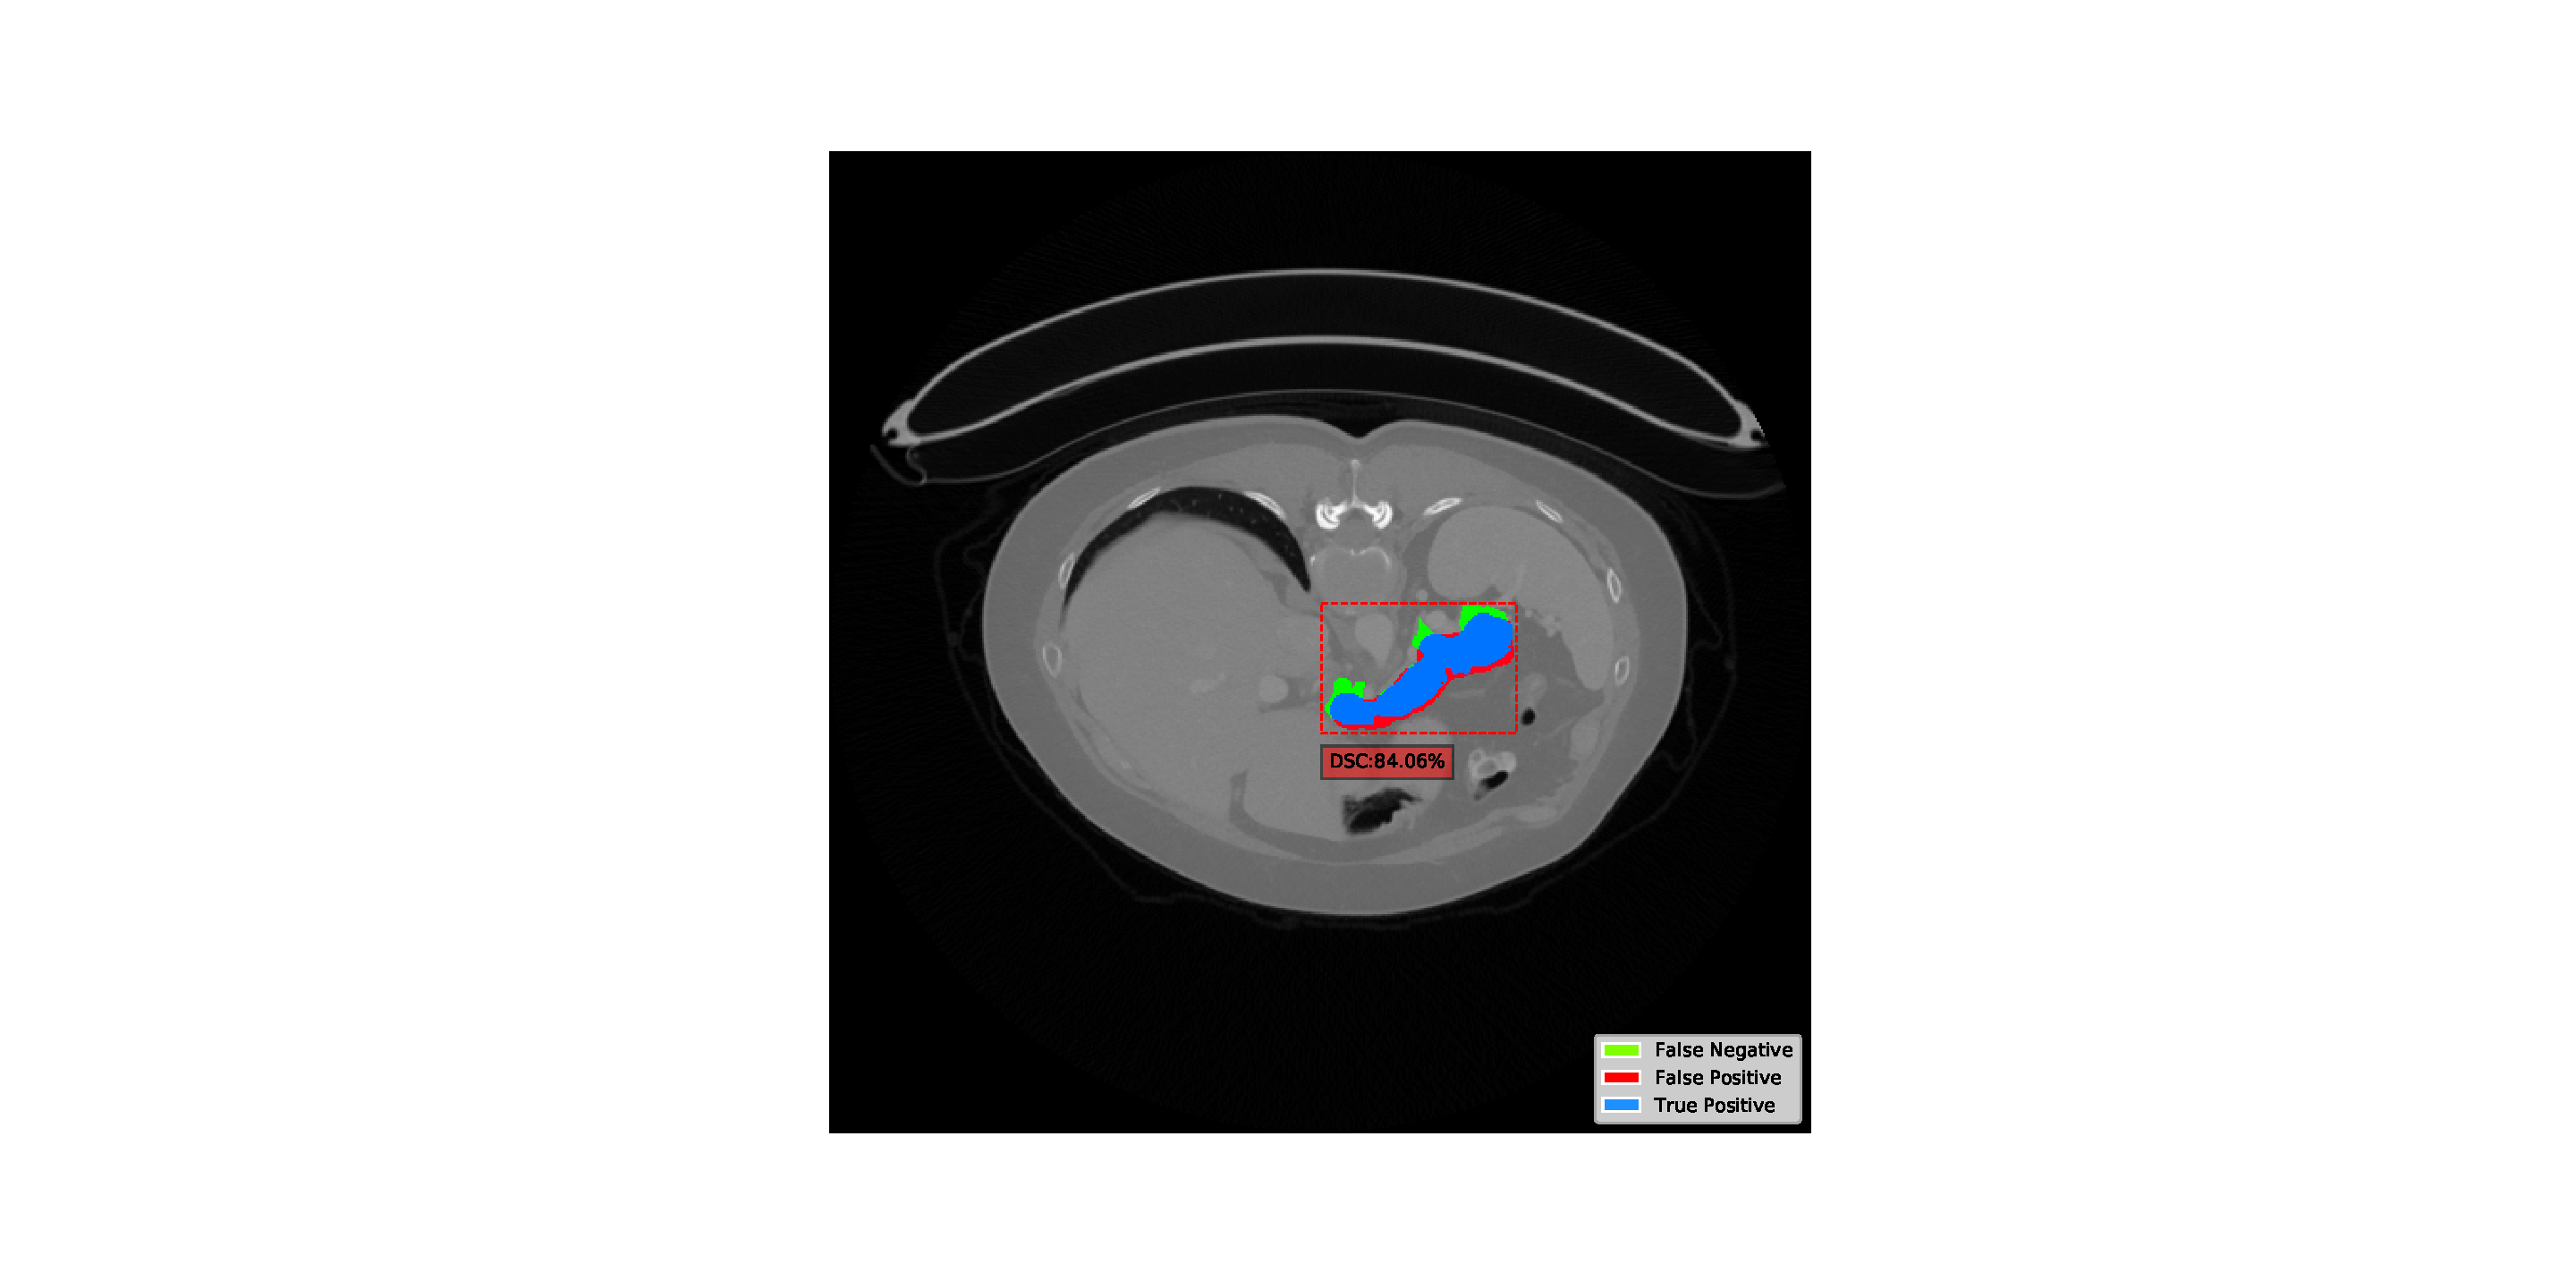
\includegraphics[width=0.425\textwidth]{Bulgular-Irdeleme/Figures/p65_slice94.pdf} & 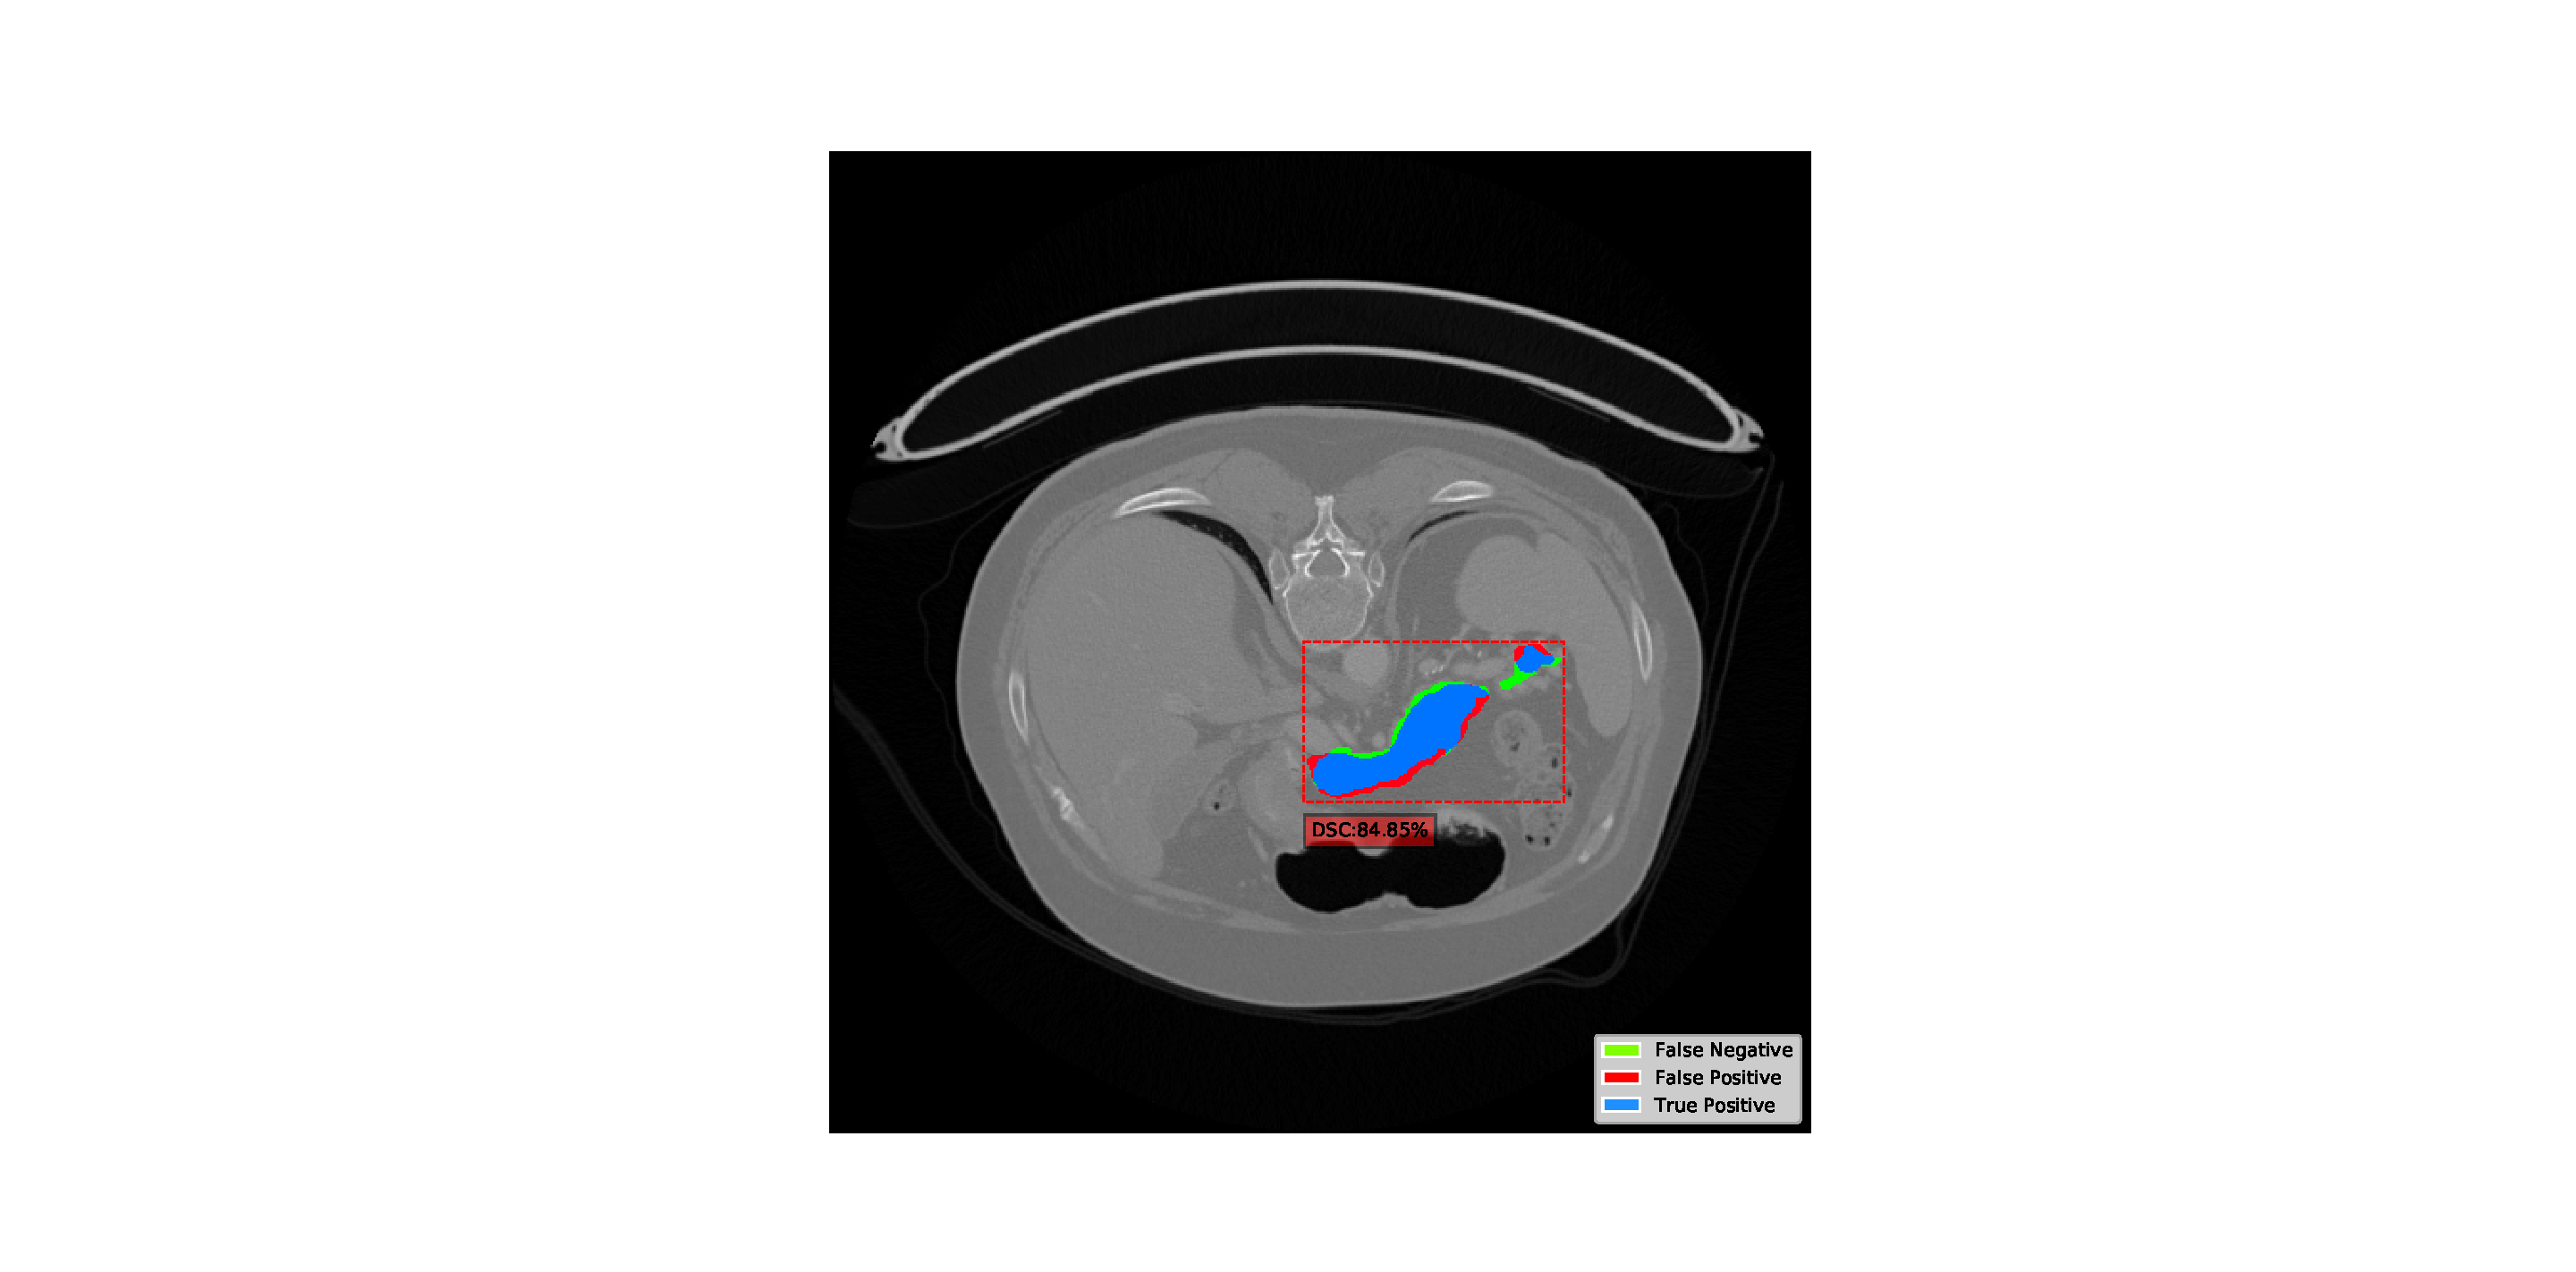
\includegraphics[width=0.425\textwidth]{Bulgular-Irdeleme/Figures/p68_slice88.pdf} \\
				(a) & (b) \\
				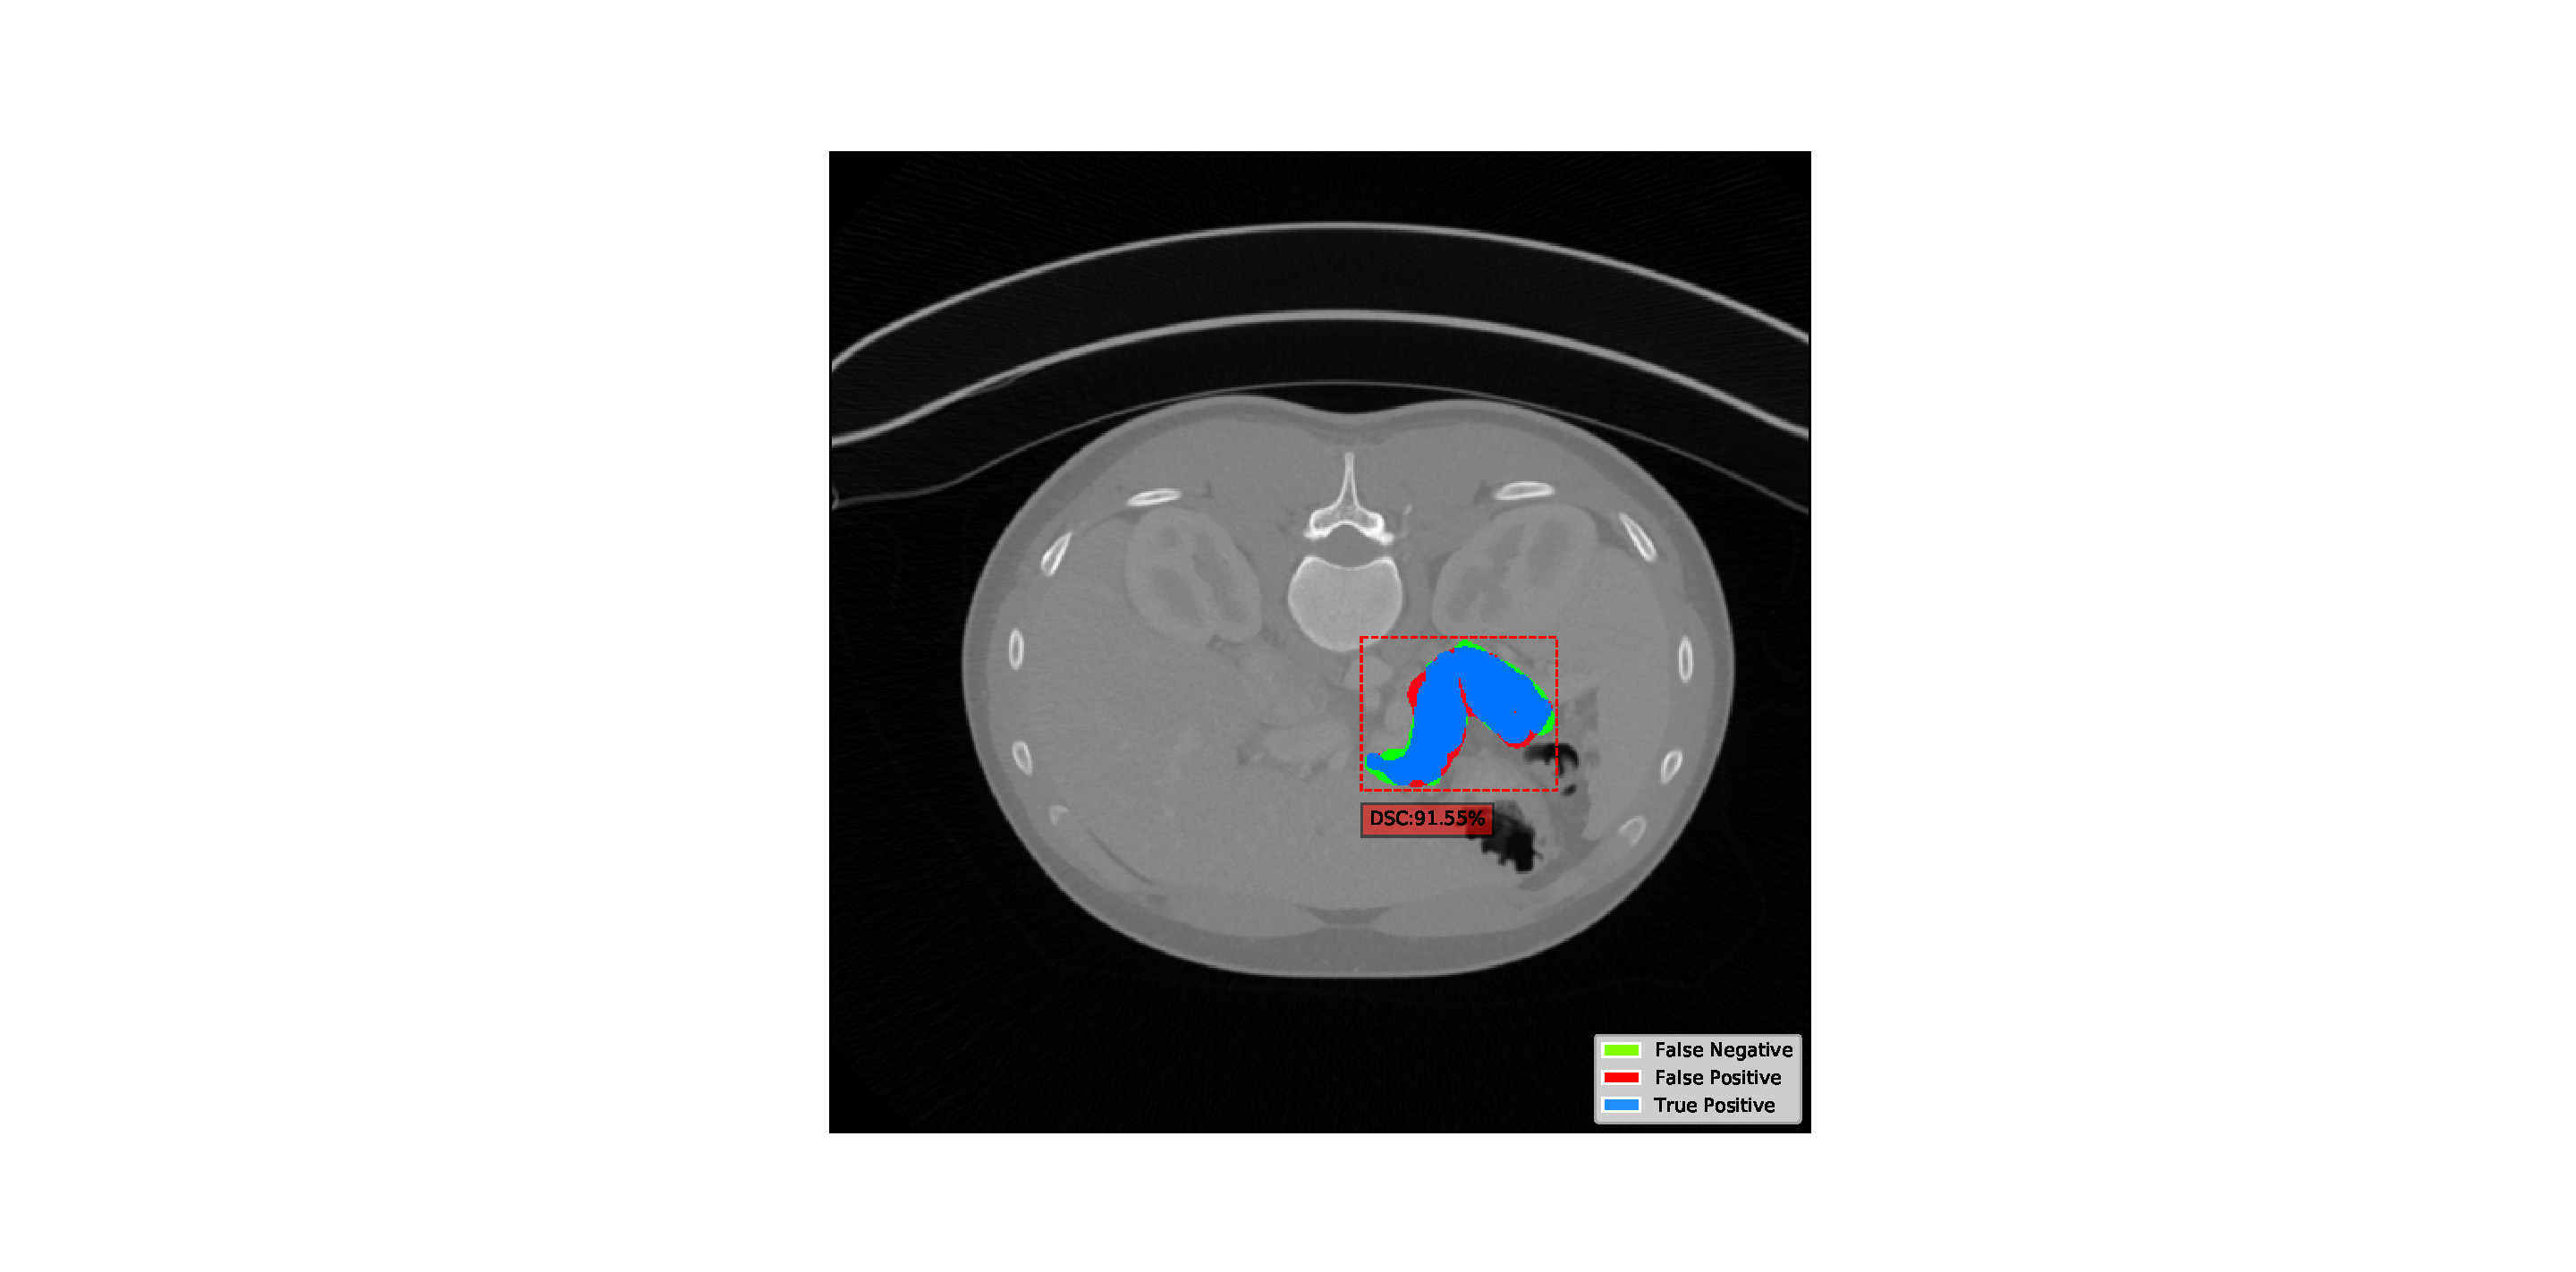
\includegraphics[width=0.425\textwidth]{Bulgular-Irdeleme/Figures/p70_slice100.pdf} & 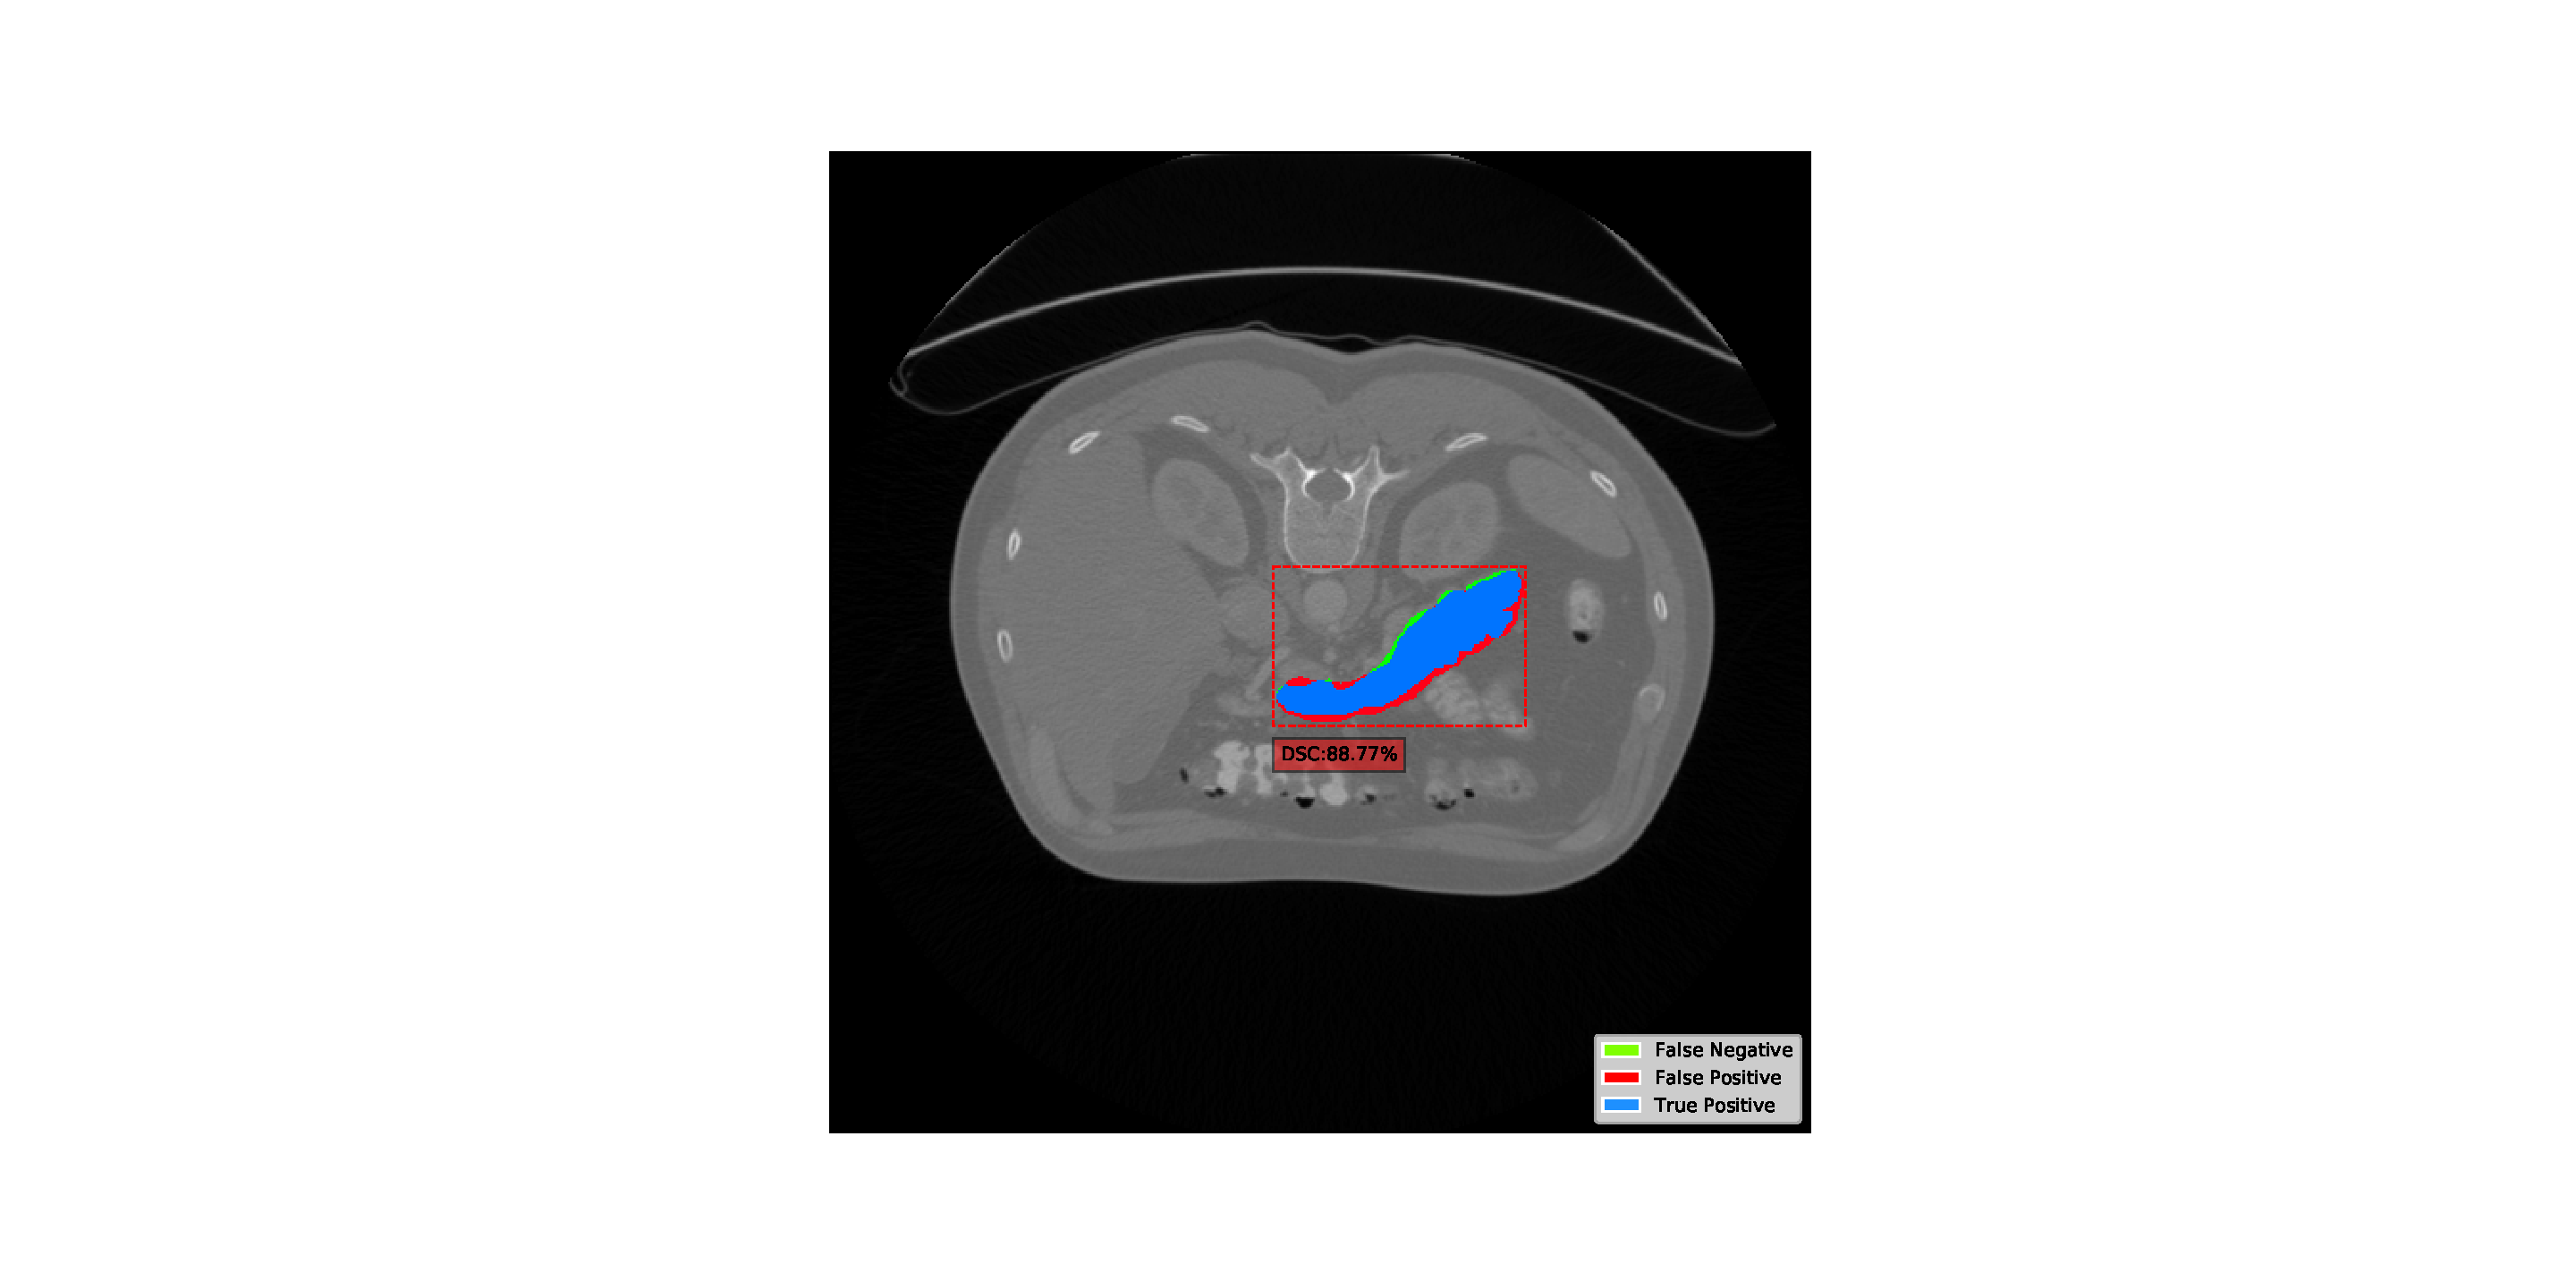
\includegraphics[width=0.425\textwidth]{Bulgular-Irdeleme/Figures/p74_slice100.pdf} \\
				(c) & (d) \\
				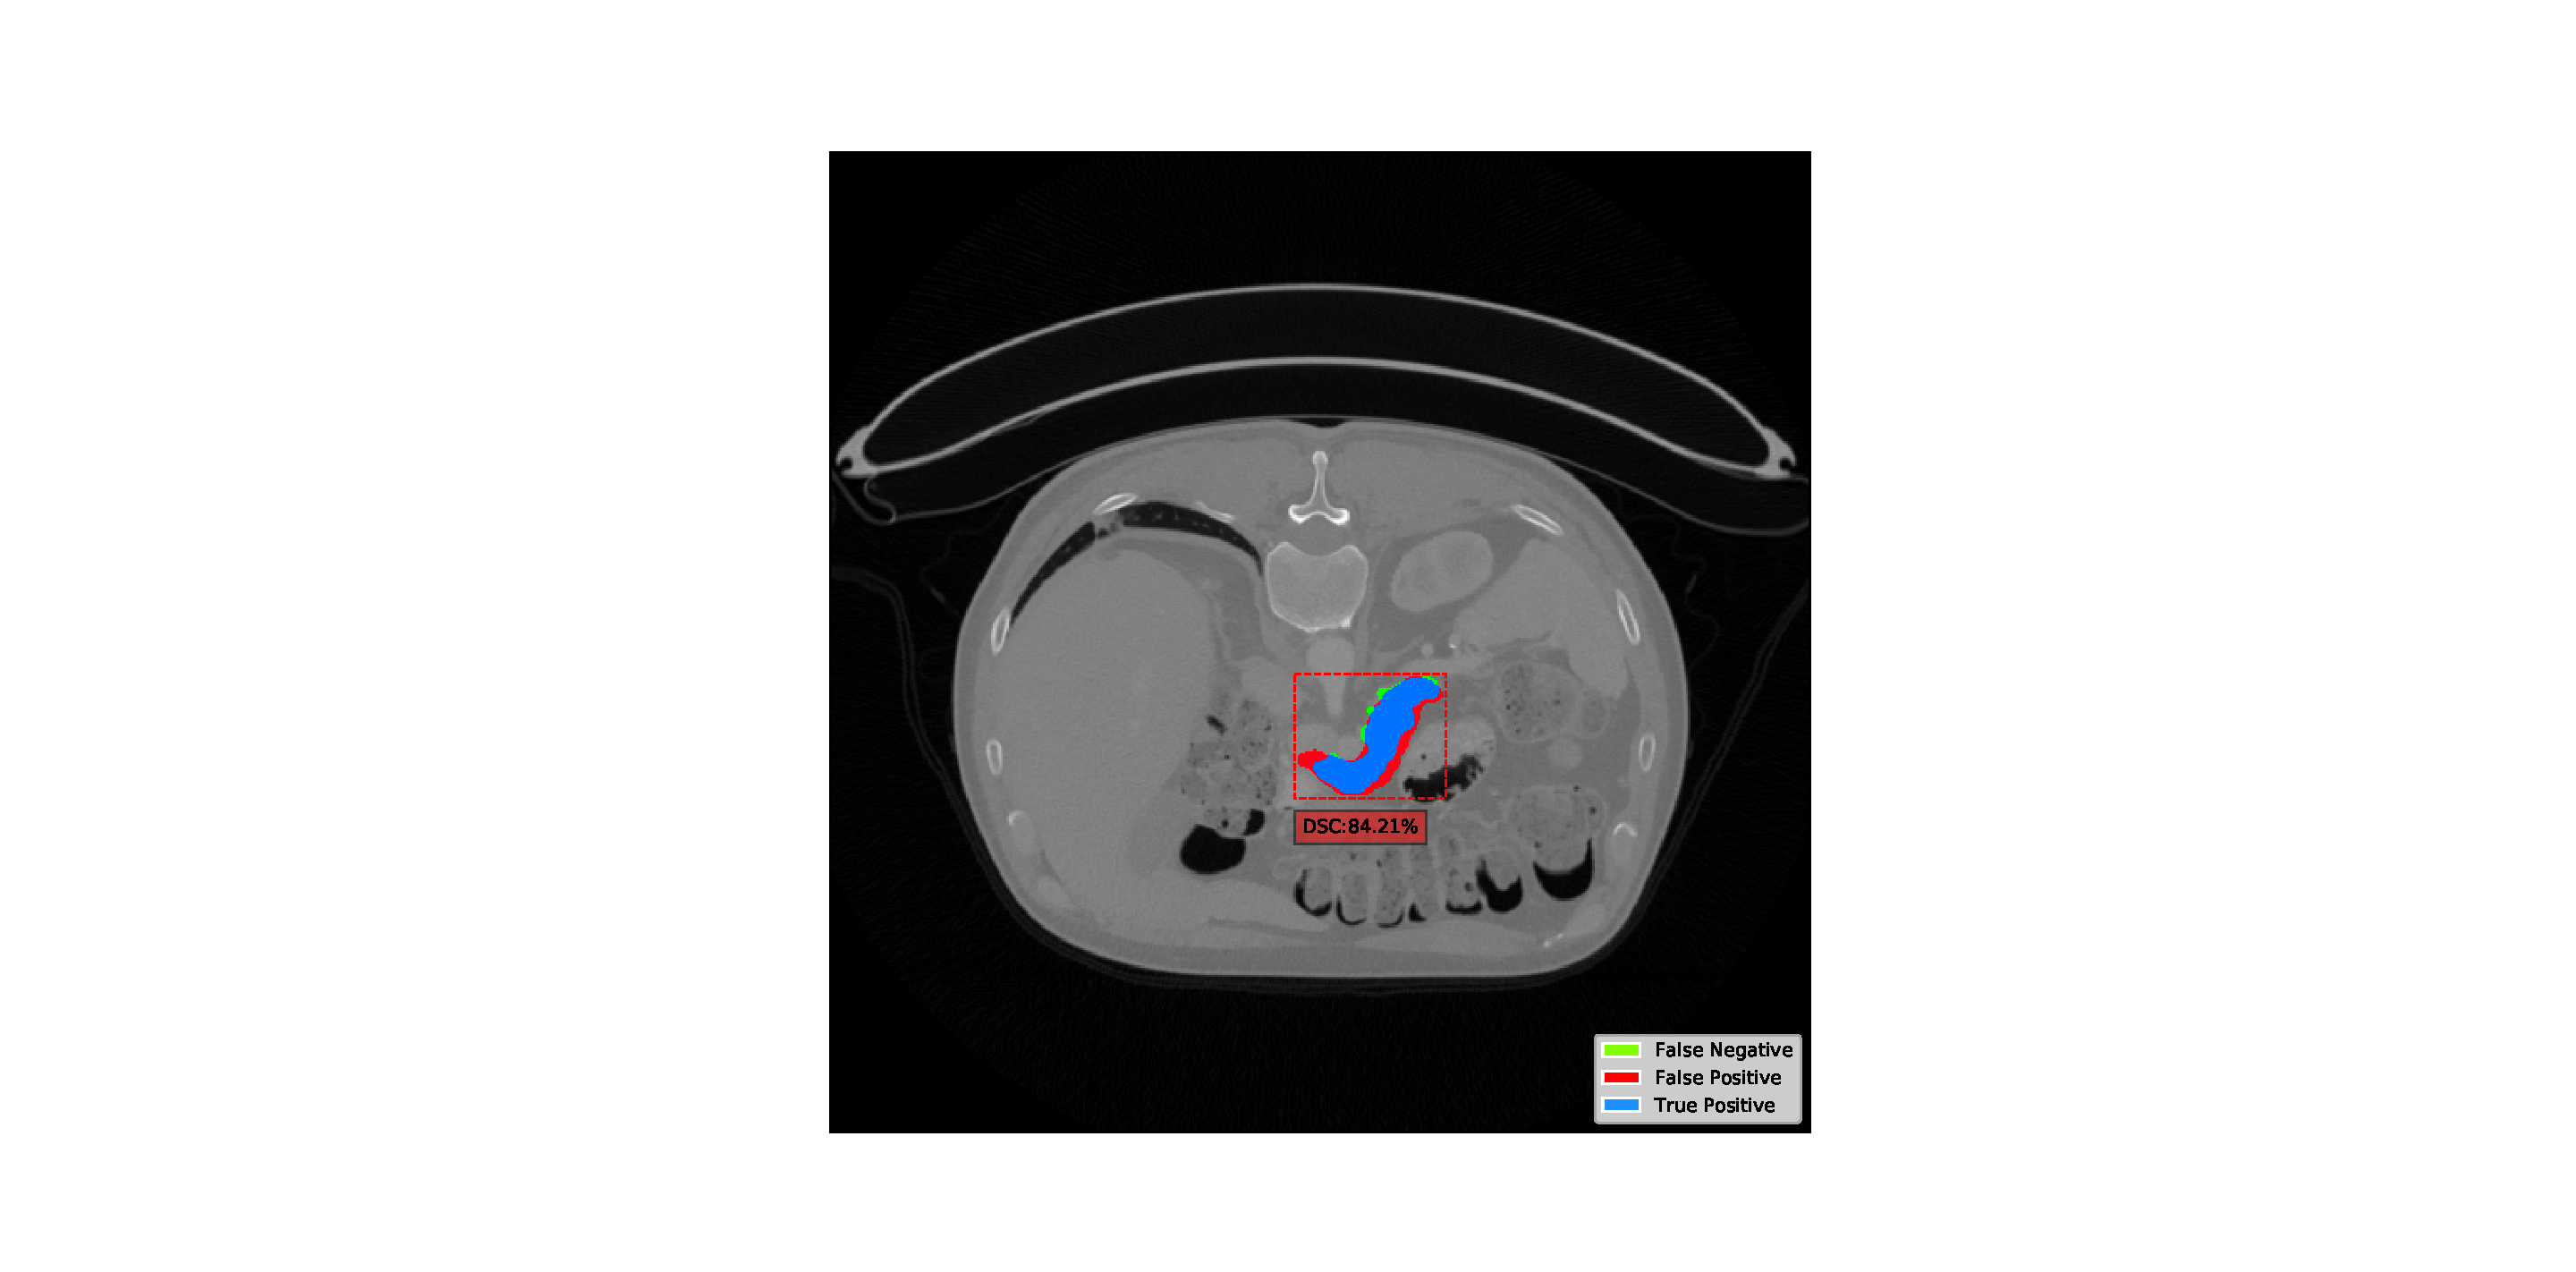
\includegraphics[width=0.425\textwidth]{Bulgular-Irdeleme/Figures/p76_slice92.pdf} & 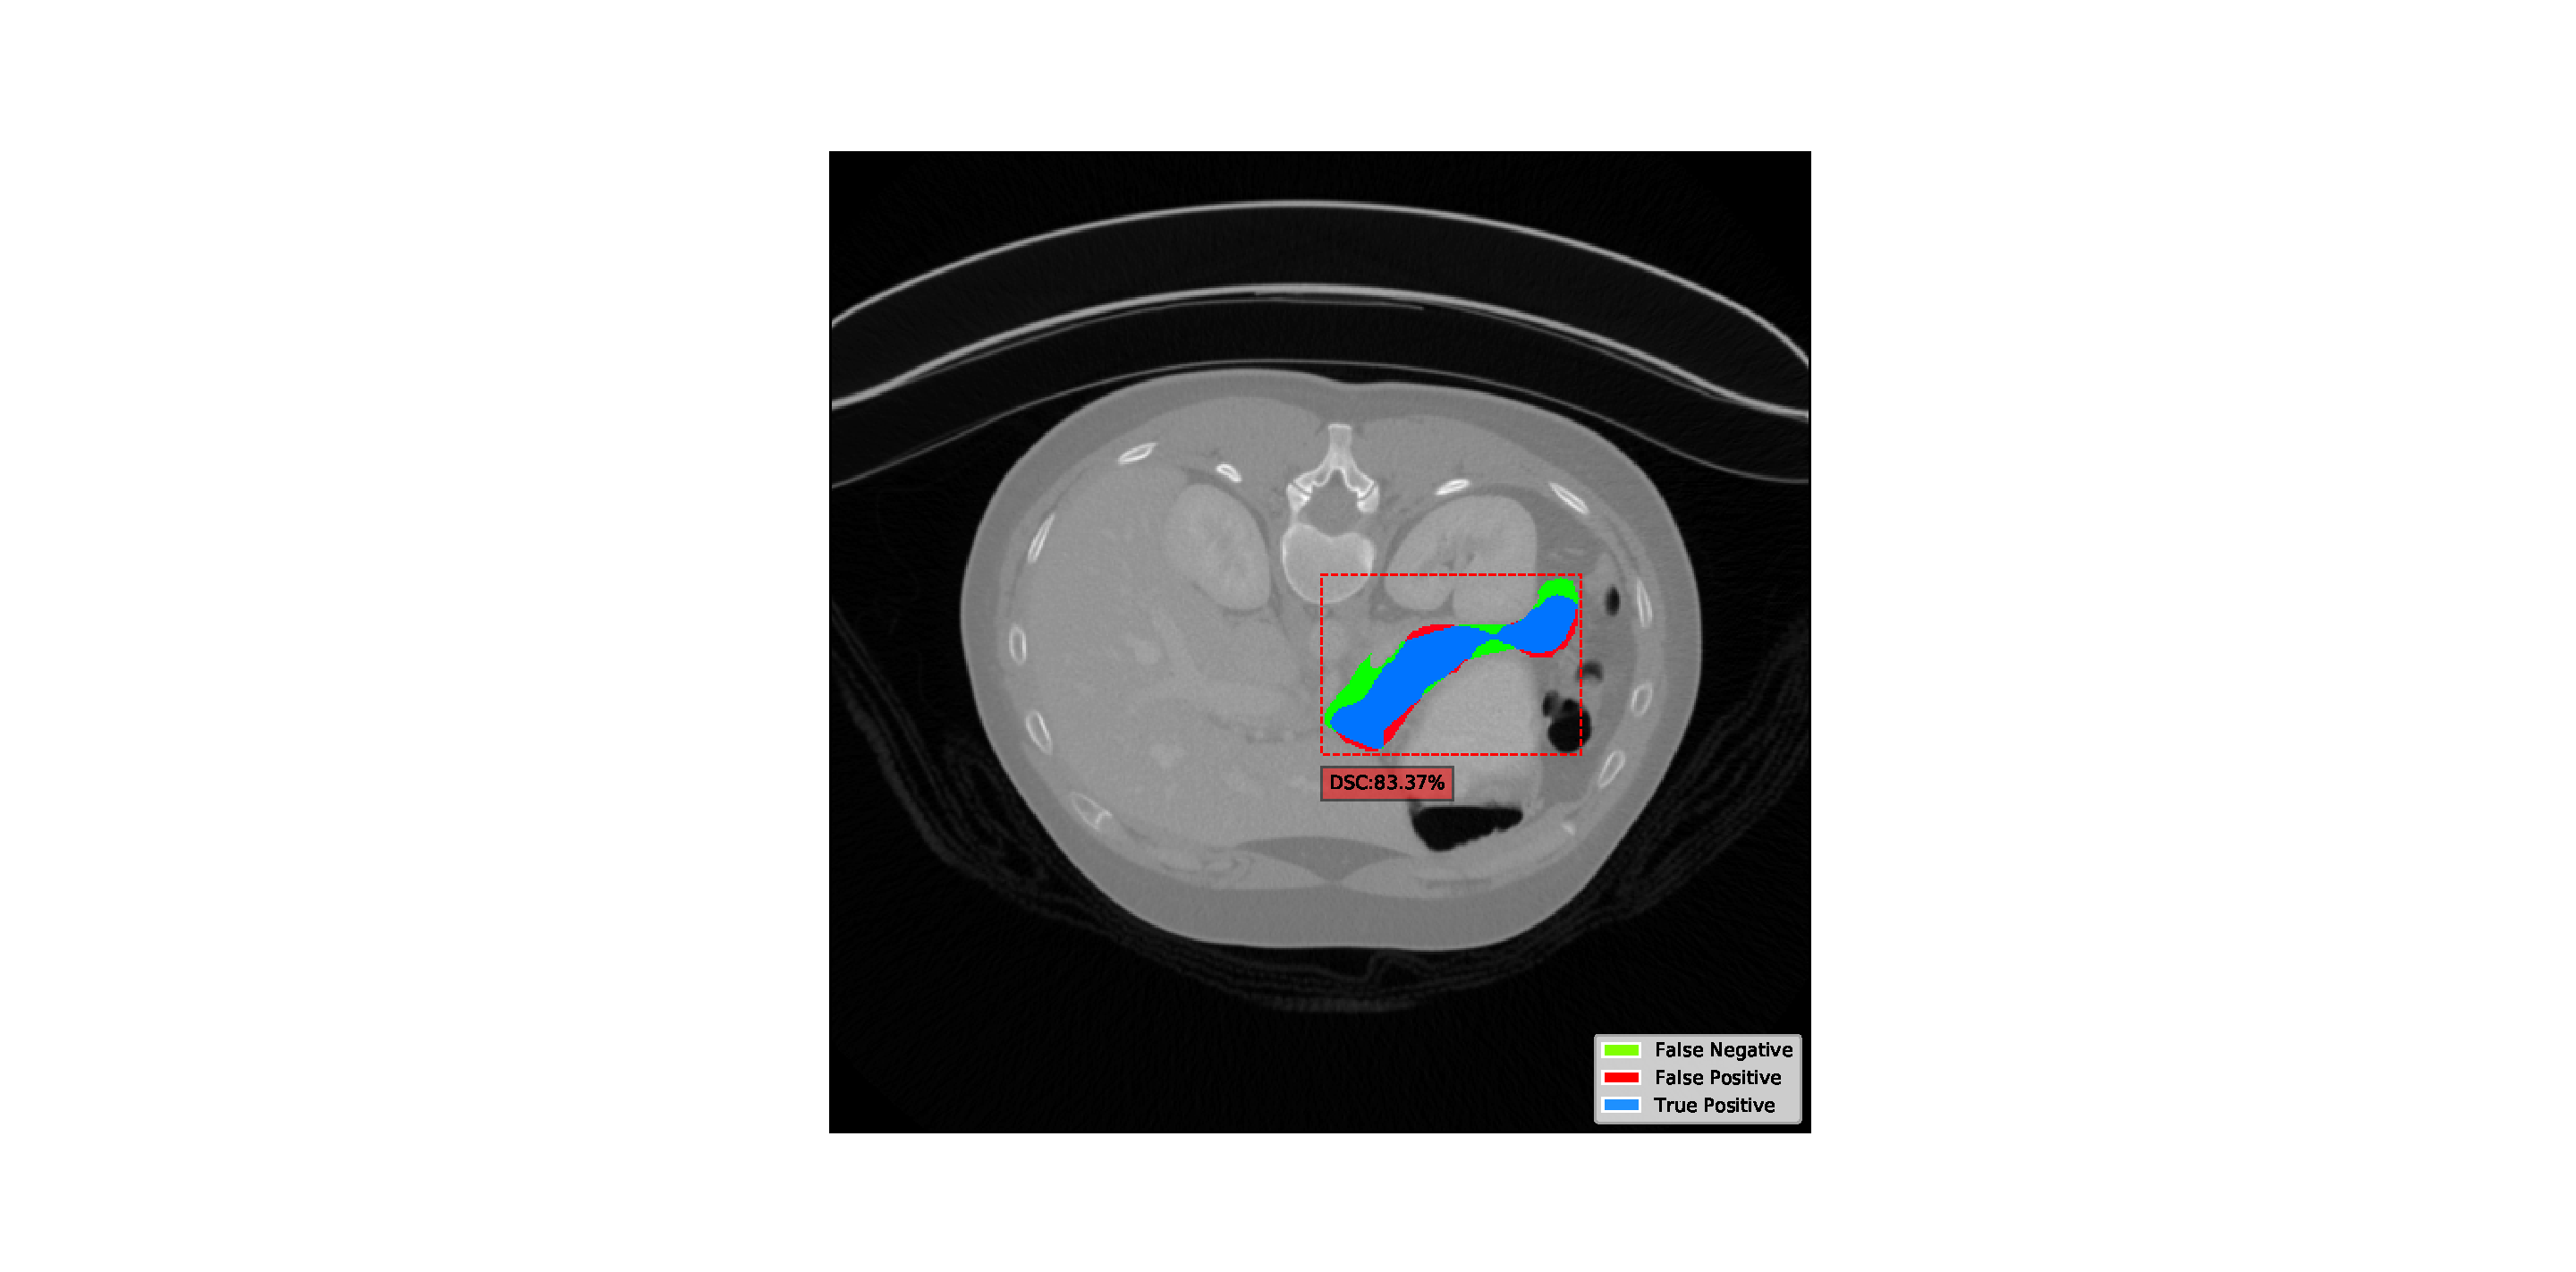
\includegraphics[width=0.425\textwidth]{Bulgular-Irdeleme/Figures/p78_slice134.pdf} \\
				(e) & (f) 
			\end{tabular}
		}
	\end{center}
\end{figure}

\captionsetup[figure]{margin={0.5cm, 0cm}}
\begin{figure}[h!]
	\begin{center}
		\vspace{0.4cm}
		\captionbox{Radyolog tarafından işaretlenen gerçek referans bölgeleri (a, b, c), önerilen iki fazlı yaklaşım (Pankreas İlgi Bölgesinin Belirlenmesi - Mask R-CNN + Pankreas Segmentasyonu  - 3B U-Net) (d, e, f), sadece birinci faz (Pankreas İlgi Bölgesinin Belirlenmesi - Mask R-CNN) (g, h, i) ve sadece ikinci faz (Pankreas Segmentasyonu - 3B U-Net) (j, k, l) kullanılarak elde edilen pankreas segmentasyon sonuçları
	    \label{fig:f1results3D}}
		{
			\begin{tabular}{ccc}
				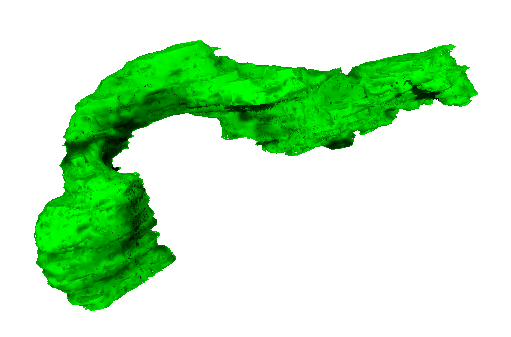
\includegraphics[width=0.3\textwidth]{Bulgular-Irdeleme/Figures/68gt3D.png} & 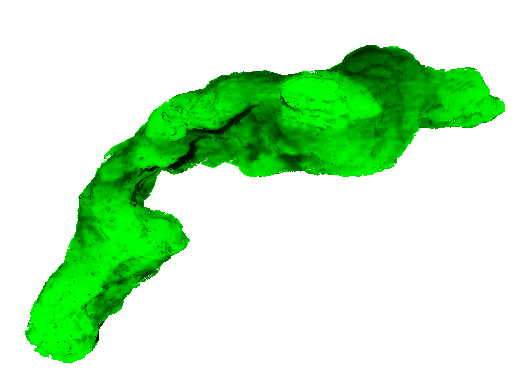
\includegraphics[width=0.3\textwidth]{Bulgular-Irdeleme/Figures/70gt3D.png} & 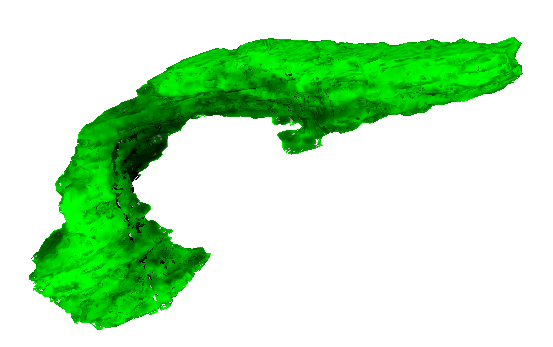
\includegraphics[width=0.3\textwidth]{Bulgular-Irdeleme/Figures/74gt3D.png} \\
				(a) & (b) & (c) \\
				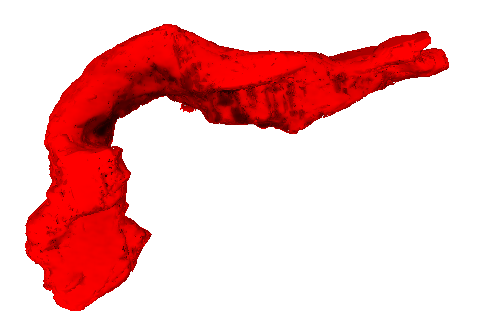
\includegraphics[width=0.3\textwidth]{Bulgular-Irdeleme/Figures/68res3D.png} & 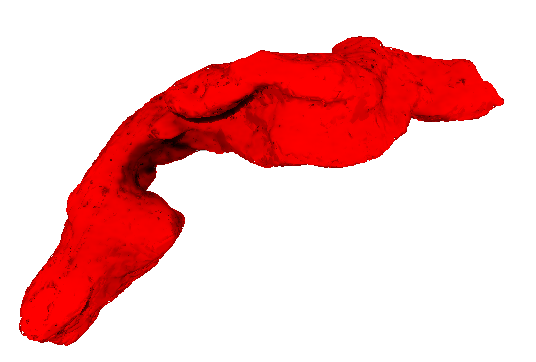
\includegraphics[width=0.3\textwidth]{Bulgular-Irdeleme/Figures/70res3D.png} & 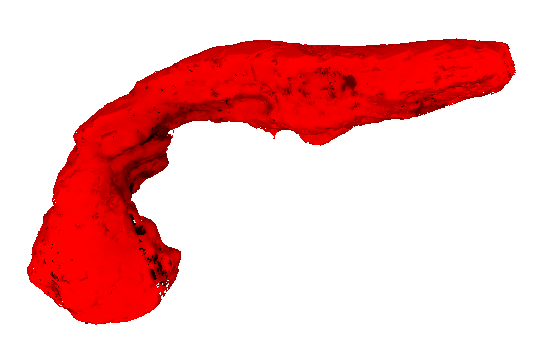
\includegraphics[width=0.3\textwidth]{Bulgular-Irdeleme/Figures/74res3D.png} \\
				(d) & (e) & (f) \\
				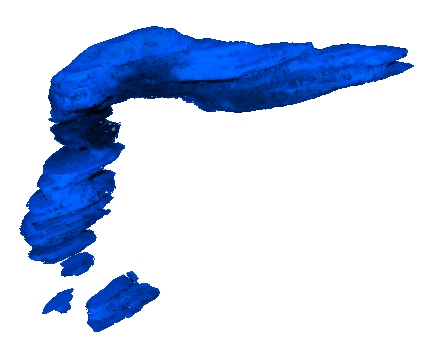
\includegraphics[width=0.3\textwidth]{Bulgular-Irdeleme/Figures/68mrcnn3D.png} & 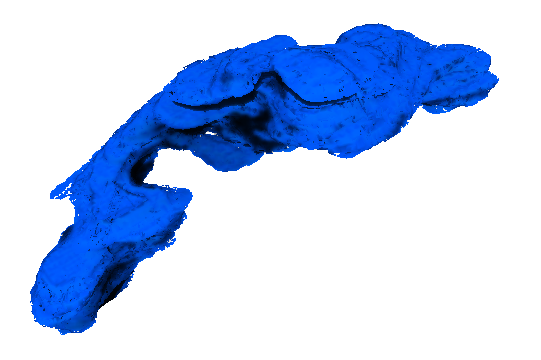
\includegraphics[width=0.3\textwidth]{Bulgular-Irdeleme/Figures/70mrcnn3D.png} & 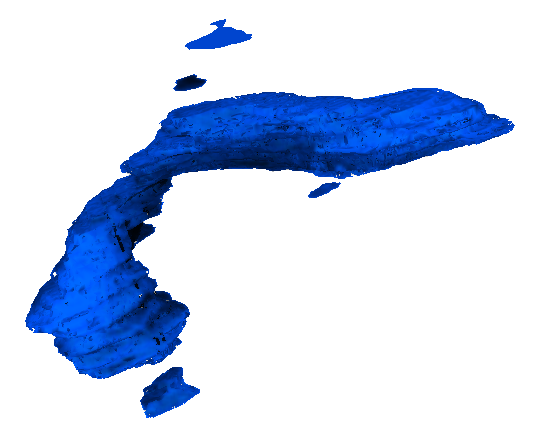
\includegraphics[width=0.3\textwidth]{Bulgular-Irdeleme/Figures/74mrcnn3D.png} \\
				(g) & (h) & (i) \\
				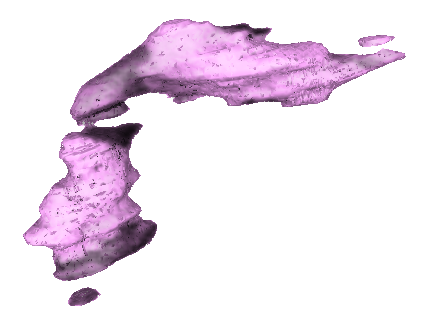
\includegraphics[width=0.3\textwidth]{Bulgular-Irdeleme/Figures/68unet3D.png} & 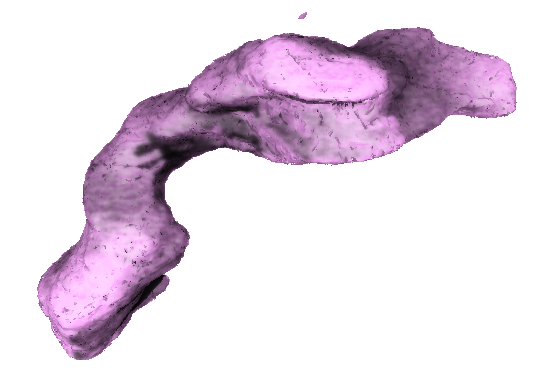
\includegraphics[width=0.3\textwidth]{Bulgular-Irdeleme/Figures/70unet3D.png} & 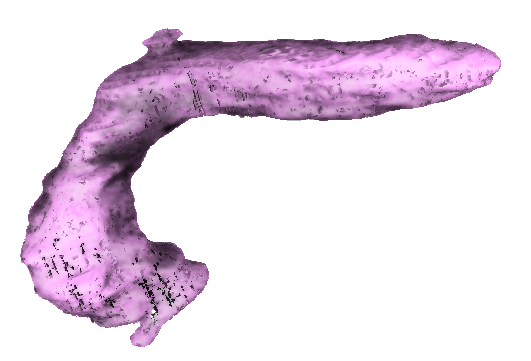
\includegraphics[width=0.3\textwidth]{Bulgular-Irdeleme/Figures/74unet3D.png} \\
				(j) & (k) & (l)
			\end{tabular}
		}
	\end{center}
\end{figure}

\section{Pankreas Segmentasyonu İçin Önerilen İki Aşamalı Yöntem için Genel Bulgular}
Bu çalışmada pankreas hastalığı bulunan kişilerin sağkalım oranını artırmak, tanı, tedavi ve cerrahide tıp doktorlarına yardımcı olmak için pankreas segmentasyonunun gerçekleştirilmesi amaçlanmaktadır. Çalışmada CNN tabanlı segmentasyon yaklaşımları önerilmektedir. Bu tez çalışmasının ilk kısmında BT görüntülemede yüksek doğrulukta otomatik pankreas segmentasyonu sağlamak için iki fazlı yeni bir yaklaşım (Pankreas İlgi Bölgesinin Belirlenmesi + Pankreas Segmentasyonu) önerilmektedir. İlk faz Pankreas İlgi Bölgesinin Belirlenmesi’dir. Bu fazda Mask R-CNN modeli uyarlanarak 2B BT dilimlerinde kaba pankreas pozisyonu tespit edilmektedir. İkinci faz ise Belirlenen İlgi Bölgesinde Pankreas Segmentasyonu’dur. Bu fazda, birinci fazda oluşturulan 2B alt BT dilimlerindeki aday pankreas bölgeleri giriş olarak alınmaktadır. 3B U-Net modeli uyarlanarak segment edilmiş pankreas bölgesi üretilmektedir. Pankreas segmentasyonu için önerilen yaklaşımın değerlendirilmesi abdominal kontrastlı pankreas BT dilimlerinden oluşan NIH veri seti kullanılarak gerçekleştirilmektedir. Performans değerlendirme metrikleri olarak Dice Benzerlik Katsayısı (Dice Similarity Coefficient - DSC), Jaccard İndeksi (Jaccard Index - JI), Kesinlik (Precision - PRE), Duyarlılık (Recall - REC), Doğruluk (Accuracy - ACC), Özgüllük (Specificity - SPE), ROC (Receiver Operating Characteristics) Eğrisi ve ROC Eğrisinin Alt Alanı (Area under the ROC Curve – AUC) tercih edilmektedir. Optimum pankreas segmentasyonu yaklaşım ile elde edilen performans değerlendirme metrikleri değerlerinin diğer yaklaşımlardan elde edilen değerlerden yüksek olması beklenmektedir. 

Sadece birinci fazın (Pankreas İlgi Bölgesinin Belirlenmesi - Mask R - CNN), sadece ikinci fazın (Pankreas Segmentasyonu – 3B U-Net) ve iki fazın (Pankreas İlgi Bölgesinin Belirlenmesi - Mask R-CNN + Pankreas Segmentasyonu – 3B U-Net) performans değerlendirme metriklerinin sonuçları sırasıyla Tablo \ref{tab:mrcnn_result}, \ref{tab:unet_result} ve \ref{tab:twop_result}'te gösterilmektedir. Tablo \ref{tab:mrcnn_result}, \ref{tab:unet_result} ve \ref{tab:twop_result}'ten elde edilen performans değerlendirme metriklerinin sonuçlarına göre önerilen iki fazlı yaklaşımın her kat için daha yüksek performans sağladığı görülmektedir. Otomatik pankreas segmentasyonu için önerilen iki fazlı yaklaşımın (Pankreas İlgi Bölgesinin Belirlenmesi - Mask R-CNN + Pankreas Segmentasyonu – 3B U-Net), DSC, JI, PRE, REC, ACC, SPE ve AUC ortalama değerleri sırasıyla \%86.15, \%75.93, \%86.23, \%86.27, \%99.95, \%99.97 ve \%99.19 olarak ölçülmektedir. Önerilen iki fazlı yaklaşım (Pankreas İlgi Bölgesinin Belirlenmesi - Mask R-CNN + Pankreas Segmentasyonu – 3B U-Net) pankreas segmentasyonunun başarısını sadece birinci faza (Pankreas Pankreas İlgi Bölgesinin Belirlenmesi - Mask R-CNN) ve sadece ikinci faza (Pankreas Segmentasyonu – 3B U-Net) göre arttırmaktadır. Performans değerlendirme metriklerinin standart sapma değerleri, önerilen yaklaşımın pankreasın farklı anatomik yapıları için kararlı segmentasyon sonuçları verdiğini göstermektedir. Önerilen yaklaşımın performans değerlendirme metriklerinin minimum değerleri \%70.49, \%54.44, \%71.25, \%69.71, \%69.71, \%99.89 ve \%99.95 olarak hesaplanmaktadır. Otomatik pankreas segmentasyonu için gerçekleştirilen literatür çalışmalarına göre yapılan tez çalışmasında kabul edilebilir segmentasyon sonuçları elde edilmektedir. Tablo \ref{tab:mrcnn_result}, \ref{tab:unet_result} ve \ref{tab:twop_result}'teki performans değerlendirme metriklerinin sayısal sonuçlarından, farklı anatomik yapılara sahip pankreasın kaba pozisyonunun belirlenmesinin (Pankreas İlgi Bölgesinin Belirlenmesi fazı), daha tatmin edici performans ile otomatik pankreas segmentasyonu için kritik bir aşama olduğu anlaşılmaktadır. Ayrıca, önerilen yaklaşımın etkinliğinin, otomatik pankreas segmentasyonu için geliştirilen literatür çalışmalarından daha üstün olduğu Tablo \ref{tab:comp_panc}'teki sonuçlardan açıkça anlaşılmaktadır.

Farklı yaklaşımlar için performans değerlendirme metriklerinden elde edilen nicel sonuçlar Tablo \ref{tab:comp_panc}'te sunulmaktadır. Literatürdeki yaklaşımlar, tez çalışmasında kullandığımız GPU'ya kıyasla daha güçlü GPU'lar ile verilerini işlemektedirler. Bu nedenle bu çalışmalar genellikle tek fazlı olup pankreas segmentasyon işlemini görüntünün tamamı üzerinde gerçekleştirmektedirler. Bizim çalışmamızda olduğu gibi daha düşük güçlü GPU'larda daha fazla performans gösterebilmek için işlenecek bölge alanını küçültmek gerekmektedir. Bu nedenle literatür çalışmalarından farklı olarak tez çalışması Pankreas İlgi Bölgesinin Belirlenmesi ve Pankreas Segmentasyonu olmak üzere iki aşamalı bir yaklaşımdan oluşmaktadır. Tablo \ref{tab:comp_panc}’teki performans değerlendirme metrikleri sonuçlarından da anlaşılacağı gibi, birinci faz (Pankreas İlgi Bölgesinin Belirlenmesi), daha güçlü GPU'lara sahip diğer yaklaşımlara göre daha düşük GPU kapasiteli tez çalışmasının başarısını olumlu yönde etkilemektedir. Performans değerlendirme metrikleri açısından, önerilen yaklaşımın etkinliğinin, otomatik pankreas segmentasyonu için gerçekleştirilen literatür çalışmalarından daha üstün olduğu açıkça görülmektedir. Önerilen yaklaşım ile DSC, JI ve REC'nin ortalama değerleri \%86.15, \%75.93 ve \%86.27 olarak üretilmektedir. Bu değerler yakın zamanda yayınlanan, \%85.99, \%75.30 ve \%86.26 değerlerine sahip yaklaşımlardan daha yüksektir. Ayrıca Tablo \ref{tab:comp_panc}'te sadece ikinci fazı (Pankreas Segmentasyonu) içeren önerilen yaklaşımımızın performans değerlendirme metrikleri sonuçlarının diğer çalışmalara göre daha düşük olduğu görülmektedir. Bunun sebebinin sahip olduğumuz GPU belleğinin diğerlerinden daha az olmasından kaynaklandığı düşünülmektedir. Ancak, daha düşük GPU kapasiteli önerilen çalışmamızın iki fazlı yaklaşım kullanarak ve işlem belleğini azaltarak daha başarılı sonuçlar elde edebileceği açıkça anlaşılmaktadır. Yüksek kapasiteli bir GPU'ya ihtiyaç duymadan yüksek performans elde edilebileceği bu tez çalışmasında kanıtlanmaktadır.

Şekil \ref{fig:f1results2D} ve \ref{fig:f1results3D}’te önerilen yaklaşımla farklı 2B görüntü ve 3B BT dilimlerinden elde edilen görsel pankreas segmentasyon sonuçları gösterilmektedir. Bu sonuçlara göre birinci faz (Pankreas İlgi Bölgesinin Belirlenmesi - Mask R-CNN) ile elde edilen kaba pankreas bölgelerinin iki aşamalı yaklaşım ile elde edilen pankreas bölgelerinin radyoloğun işaretlediği pankreas bölgelerine daha benzer olmalarını sağladığı gözükmektedir. Birinci faz (Pankreas İlgi Bölgesinin Belirlenmesi - Mask R-CNN) ile elde edilen kaba pankreas bölgeleri, iki fazlı yaklaşım ile elde edilen pankreas bölgelerine göre daha dağınıktır. Ek olarak, bu kaba pankreas bölgeleri radyoloğun işaretlediği pankreas bölgelerine daha az benzerdir. Yapılan tez çalışmasında ilk fazla (Pankreas İlgi Bölgesinin Belirlenmesi - Mask R-CNN) kaba pankreas bölgesinin bulunması, pankreas segmentasyonu için ikinci aşamada tüm görüntüyü işleyen diğer literatür çalışmalarına göre daha az güç ve zaman karmaşıklığı sağlamaktadır. Tüm görüntüyü işleyen 3B U-Net yaklaşımıyla karşılaştırıldığında, iki fazlı yaklaşım daha belirgin kavisli bölgeler çıkarmaktadır. Bu bölgeler radyolog tarafından işaretlenen pankreas bölgelerine daha çok benzemektedir. İlk faz (Pankreas İlgi Bölgesinin Belirlenmesi -  Mask R-CNN) pankreas bölgelerinde 3B U-Net'ten daha fazla artifaktlı segmentlere ayırmaktadır. Fakat ilk faz (Pankreas İlgi Bölgesinin Belirlenmesi - Mask R-CNN) tarafından segmentlere ayrılan pankreas bölgeleri radyolog tarafından işaretlenen pankreas bölgelerine daha çok benzemektedir.

\section{Pankreas ve Pankreas Tümörü Segmentasyonu İçin Önerilen İki Aşamalı Yöntemin Farklı Derin Öğrenme Teknikleri ile İncelenmesine Yönelik Deneysel Sonuçlar}

Bu tez çalışmasında pankreas segmentasyonu için önerilen iki aşamalı segmentasyon yöntemi pankreas ve pankreas tümörlerinin işaretlendiği MSD pankreas veri seti üzerinde yeniden ele alınmaktadır. Bu bağlamda bu bölümde farklı derin ağ modellerinin performansının önerilen iki aşamalı yönteme etkileri üzerinde durulmaktadır.

\subsection{Önerilen Ağ Mimarilerinin Özellikleri}
Pankreas ve pankreas tümörü segmentasyonu kısmının ilk fazı olan Pankreas İlgi Bölgesinin Belirlenmesi’nde, pankreas segmentasyonu kısmında olduğu gibi Waleed Abdulla tarafından geliştirilen Keras ve Tensorflow tabanlı Mask R-CNN modeli \cite{he2017mask} kullanılmaktadır. Pankreas ve pankreas tümörü segmentasyonu kısmında Mask R-CNN yönteminde Çekirdek Ağı olarak ResNet-50 ve ResNet-101 modelleri ayrı ayrı kullanılmaktadır. Pankreas İlgi Bölgesinin Belirlenmesi fazının farklı çekirdek ağları ile performansı irdelenmektedir. 

Pankreas ve pankreas tümörü segmentasyonu kısmının ikinci fazı olan Pankreas ve Pankreas Tümörü Segmentasyonu’nda, önceki fazda (Pankreas İlgi Bölgesinin Belirlenmesi) elde edilen alt BT görüntülerinde pankreas ve pankreas tümörü segmentasyonu gerçekleştirilmektedir. Bu amaçla Pankreas ve Pankreas Tümörü Segmentasyonu fazında 3B Standart FCN Oto Kodlayıcı, 3B UNet, 3B UNet++ olmak üzere üç farklı segmentasyon modeli ayrı ayrı kullanılmaktadır. Pankreas ve Pankreas Tümörü Segmentasyonu fazı için farklı segmentasyon modellerinin performansı incelenmektedir.

Pankreas ve pankreas tümörü segmentasyonu kısmındaki Pankreas İlgi Bölgesinin Belirlenmesi ve Pankreas Tümörü Segmentasyonu fazlarının eğitim ve test süreçleri için standart çapraz doğrulama stratejisi kullanılmaktadır. MSD veri setinin (282 hasta) rastgele bölünmesinde dört kat (fold) çapraz doğrulama gerçekleştirilmektedir. Tasarlanan modellerin eğitim iterasyonları her kat için 100.000'de durdurulmaktadır. Otomatik pankreas ve pankreas tümörü segmentasyonu için tasarlanan Pankreas İlgi Bölgesinin Belirlenmesi ve Pankreas Tümörü Segmentasyonu fazlarının eğitim süreleri sırasıyla yaklaşık 10 ve 1,5 gün sürmektedir. Pankreas İlgi Bölgesinin Belirlenmesi ve Pankreas Tümörü Segmentasyonu fazlarının test süreçlerinde ise bir BT dilimi için ortalama çalışma süresi yaklaşık 20 saniye olarak hesaplanmaktadır.

\subsection{Pankreas İlgi Bölgesinin Belirlenmesi Fazında Farklı Çekirdek Ağlarının Etkisi}

\captionsetup[figure]{margin={0.3cm,0cm}}
\begin{figure}[h!]
	\begin{center}
		\vspace{0.4cm}
		\captionbox{ResNet-50 ve ResNet-101 mimarileri için çekirdek ağı performans karşılaştırması.\label{fig:center_distance}}
		{
			\vspace{0.4cm}
			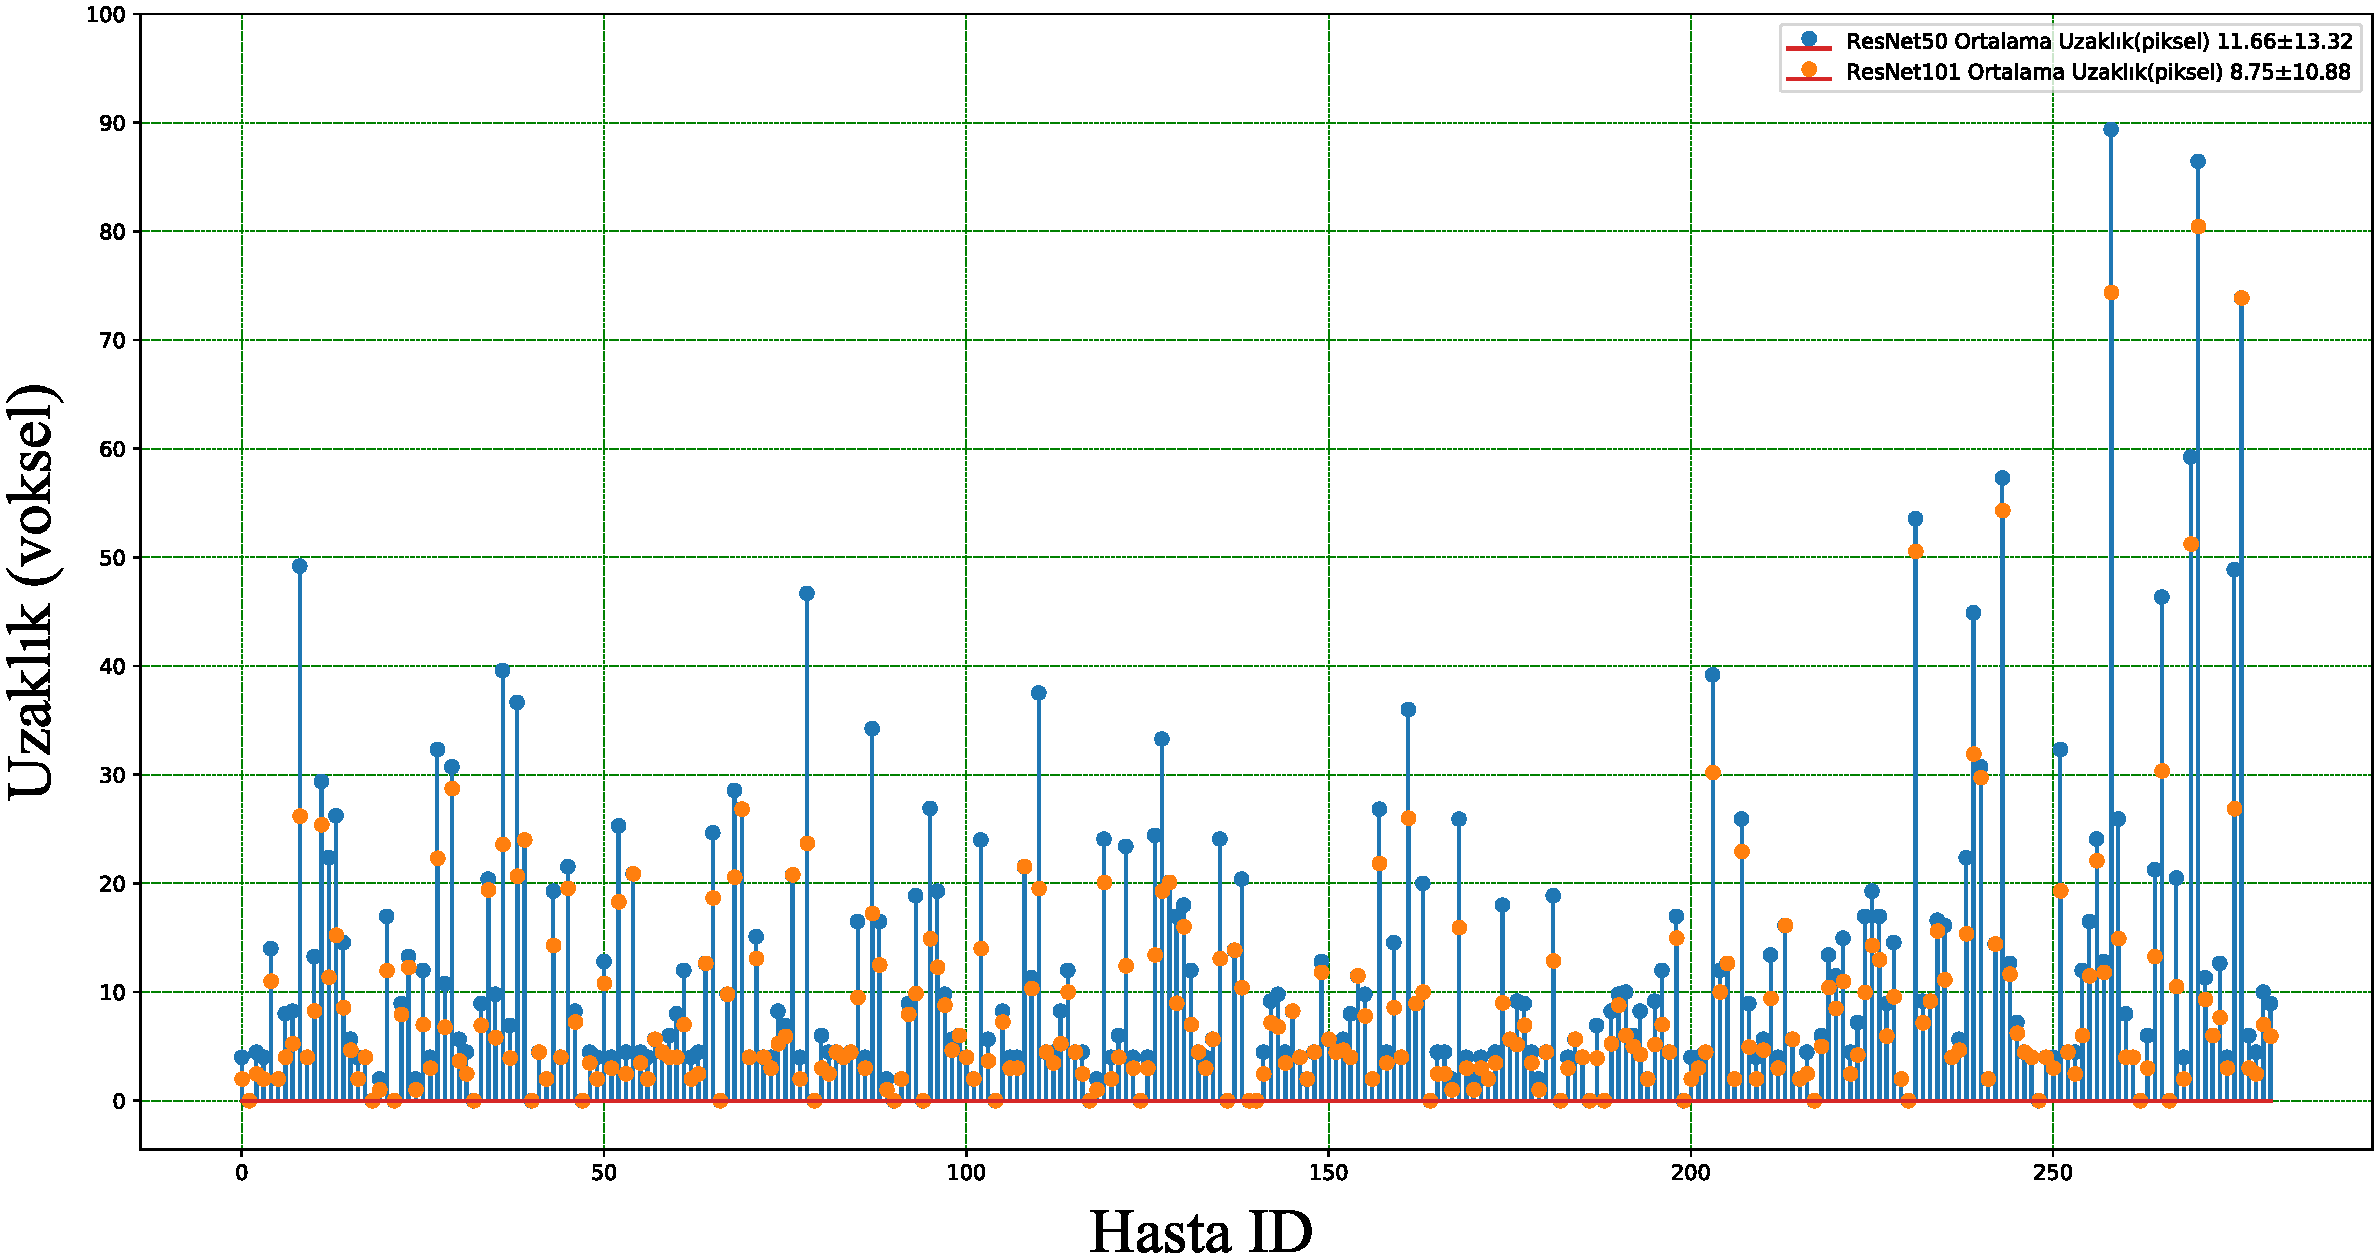
\includegraphics[scale=0.38]{Bulgular-Irdeleme/Figures/center_distance.pdf}
		}
	\end{center}
\end{figure}

Pankreas İlgi Bölgesinin Belirlenmesi fazının performansında çekirdek ağının etkilerini irdelenmek amacıyla ResNet-50 ve ResNet-101 modelleri ayrı ayrı denenmektedir. ResNet-50 ve ResNet-101 modelleri ayrı ayrı çekirdek ağı olarak ImageNet ağırlıkları kullanılarak eğitilmektedir. 3B kesin referans volümetrik pankreas maskesi verisinin ağırlık merkezleri ($A$), ResNet-50 ve ResNet-101 modellerinin ürettiği 3B volümetrik maskelerin ağırlık merkezlerinin uzaklıkları ($B$) ve her bir ağırlık merkezi 3B uzayda ($x,y,z$) şeklinde bir noktayı (voksel) temsil etmek üzere $|AB|$ uzaklığı Eşitlik \ref{eq:center_distance}'deki gibi hesaplanmaktadır.
\begin{equation}
	\label{eq:center_distance}
	|AB|=\sqrt{\left(x_{2}-x_{1}\right)^{2}+\left(y_{2}-y_{1}\right)^{2}+\left(z_{2}-z_{1}\right)^{2}}
\end{equation}

Şekil \ref{fig:center_distance}’te ResNet-50 ve ResNet-101 mimarileri için çekirdek ağı performans karşılaştırması gösterilmektedir. ResNet-101 modelinin ortalama uzaklık değeri 8.75 iken ResNet-50 modelinin ortalama uzaklık değeri 11.66 olarak ölçülmektedir. Elde edilen sonuçlara göre ResNet-101 modeli çekirdek ağı olarak kullanıldığında her bir hasta için Pankreas İlgi Bölgesinin Belirlenmesi fazının çok daha başarılı pankreas konum bilgisi ürettiği görülmektedir.

\subsection{Pankreas ve Pankreas Tümörü Segmentasyonu İçin Önerilen İki Aşamalı Yöntemin Farklı Derin Öğrenme Teknikleri ile İncelenmesine Dair Elde Edilen Sayısal Sonuçlar}

Çalışmamızın ikinci kısmında yüksek doğruluklu, daha detaylı pankreas ve pankreas tümörü segmentasyonu gerçekleştirmek amaçlanmaktadır. Bu kapsamda tez çalışmasının ikinci kısmının ikinci fazı olan Pankreas ve Pankreas Tümörü Segmentasyonunda 3B FCN Oto Kodlayıcı, 3B U-Net ve 3B U-Net++ modelleri ayrı ayrı denenmektedir. İkinci fazda (Pankreas ve Pankreas Tümörü Segmentasyonu) kullanılan modellerin karşılaştırılması ve elde edilen sonuçları daha objektif değerlendirmek için 3B FCN Oto Kodlayıcı, 3B U-Net ve 3B U-Net++ modellerinin segmentasyon sonuçları ayrı ayrı verilmektedir. Pankreas ve Pankreas Tümörü Segmentasyonu için Standart 3B FCN Oto Kodlayıcı, 3B U-Net ve 3B U-Net++ modellerinin kullanılması durumunda performans değerlendirme metriklerinin sonuçları sırasıyla Tablo \ref{tab:p2autoencoderp}, \ref{tab:p2autoencodert}, \ref{tab:p2unetp}, \ref{tab:p2unett}, \ref{tab:p2unet++p} ve \ref{tab:p2unet++t}'de gösterilmektedir.

\begin{sidewaystable}[htpb]
	\centering
	\caption{Pankreas Segmentasyonu için 3B FCN Oto Kodlayıcı modelinin kullanılması durumunda performans değerlendirme metriklerinin sonuçları (Ortalama$\pm$STD[MIN,MAK])}
	\label{tab:p2autoencoderp}
	\begin{adjustbox}{width=\textwidth}		
		\begin{tabular}{ccccccc}
			\toprule
			Kat   &  DSC \%       &  JI  \%   &  PRE  \%   &  REC  \%  & ACC  \%  &  SPE  \% \\ 
			\midrule 
			1 & 77.10$\pm$7.32[58.45,86.49] & 63.25$\pm$9.16[41.29,76.19] & 77.04$\pm$7.07[60.95,85.70] & 77.43$\pm$8.63[52.33,87.66] & 99.94$\pm$0.01[99.92,99.96] & 99.97$\pm$0.01[99.96,99.98] \\
            2 & 76.29$\pm$7.68[57.41,84.96] & 62.24$\pm$9.68[40.26,73.86] & 77.65$\pm$6.78[62.55,85.13] & 75.34$\pm$9.52[48.38,88.55] & 99.94$\pm$0.02[99.91,99.96] & 99.97$\pm$0.01[99.95,99.98] \\
            3 & 77.77$\pm$6.04[60.11,85.75] & 63.99$\pm$7.60[42.97,75.05] & 78.22$\pm$6.47[58.89,85.05] & 77.39$\pm$5.97[61.39,86.72] & 99.95$\pm$0.02[99.91,99.97] & 99.98$\pm$0.01[99.95,99.99] \\
            4 & 77.80$\pm$6.32[58.57,85.91] & 64.06$\pm$8.06[41.41,75.30] & 78.38$\pm$5.75[59.79,84.56] & 77.39$\pm$7.72[57.40,88.02] & 99.94$\pm$0.01[99.90,99.96] & 99.97$\pm$0.01[99.95,99.98] \\
			\toprule
			Ortalama  & 77.24$\pm$6.84[57.41,86.49] & 63.39$\pm$8.63[40.26,76.19] & 77.82$\pm$6.52[58.89,85.70] & 76.89$\pm$7.96[48.38,88.55] & 99.95$\pm$0.02[99.90,99.97] & 99.97$\pm$0.01[99.95,99.99] \\
            \bottomrule			
		\end{tabular}
	\end{adjustbox}
	\vspace{2\baselineskip}
	\caption{Pankreas Tümörü Segmentasyonu için 3B FCN Oto Kodlayıcı modelinin kullanılması durumunda performans değerlendirme metriklerinin sonuçları (Ortalama$\pm$STD[MIN,MAK])}
	\label{tab:p2autoencodert}
	\begin{adjustbox}{width=\textwidth}		
		\begin{tabular}{ccccccc}
			\toprule
			Kat   &  DSC \%       &  JI  \%   &  PRE  \%   &  REC  \%  & ACC  \%  &  SPE  \% \\ 
			\midrule 
			1 & 48.43$\pm$7.02[32.32,69.47] & 32.24$\pm$6.41[19.28,53.22] & 51.94$\pm$8.42[33.71,74.27] & 45.76$\pm$7.26[31.04,65.25] & 99.93$\pm$0.02[99.89,99.96] & 99.97$\pm$0.01[99.95,99.98] \\
            2 & 47.62$\pm$6.24[30.70,64.20] & 31.46$\pm$5.45[18.13,47.27] & 51.14$\pm$6.58[42.87,69.47] & 44.96$\pm$6.79[23.28,59.67] & 99.93$\pm$0.01[99.89,99.96] & 99.97$\pm$0.01[99.95,99.98] \\
            3 & 49.01$\pm$6.09[32.61,66.81] & 32.67$\pm$5.49[19.48,50.16] & 52.54$\pm$7.76[38.15,71.86] & 46.31$\pm$6.35[28.48,62.42] & 99.93$\pm$0.02[99.89,99.96] & 99.97$\pm$0.01[99.95,99.98] \\
            4 & 49.02$\pm$6.46[31.01,68.51] & 32.70$\pm$5.86[18.35,52.10] & 52.56$\pm$7.67[33.22,73.41] & 46.27$\pm$6.73[29.08,64.23] & 99.93$\pm$0.01[99.89,99.96] & 99.97$\pm$0.01[99.95,99.98] \\
			\toprule
			Ortalama & 48.52$\pm$6.45[30.70,69.47] & 32.27$\pm$5.80[18.13,53.22] & 52.05$\pm$7.61[33.22,74.27] & 45.82$\pm$6.78[23.28,65.25] & 99.93$\pm$0.02[99.89,99.96] & 99.97$\pm$0.01[99.95,99.98] \\		
			\bottomrule			
		\end{tabular}
	\end{adjustbox}	
\end{sidewaystable}

\begin{sidewaystable}[htpb]
	\centering
	\caption{Pankreas Segmentasyonu için Standart 3B U-Net modelinin kullanılması durumunda performans değerlendirme metriklerinin sonuçları (Ortalama$\pm$STD[MIN,MAK])}
	\label{tab:p2unetp}
	\begin{adjustbox}{width=\textwidth}		
		\begin{tabular}{ccccccc}
			\toprule
			Kat   &  DSC \%       &  JI  \%   &  PRE  \%   &  REC  \%  & ACC  \%  &  SPE  \% \\ 
			\midrule 
			1 & 80.37$\pm$5.09[64.80,87.51] & 67.46$\pm$6.73[47.93,77.79] & 80.77$\pm$5.16[66.74,91.70] & 80.16$\pm$6.37[62.98,89.02] & 99.95$\pm$0.01[99.92,99.97] & 99.97$\pm$0.01[99.96,99.99] \\
            2 & 80.08$\pm$5.27[64.63,88.37] & 67.08$\pm$7.07[47.74,79.17] & 81.38$\pm$5.11[68.79,89.20] & 79.00$\pm$6.43[60.94,87.66] & 99.95$\pm$0.02[99.91,99.96] & 99.98$\pm$0.01[99.95,99.98] \\
            3 & 79.61$\pm$5.01[65.54,86.76] & 66.39$\pm$6.62[48.74,76.62] & 80.11$\pm$4.84[68.61,86.97] & 79.21$\pm$5.81[60.31,87.02] & 99.95$\pm$0.01[99.92,99.97] & 99.97$\pm$0.01[99.95,99.99] \\
            4 & 80.05$\pm$5.52[63.44,86.86] & 67.06$\pm$7.26[46.46,76.77] & 80.16$\pm$5.98[59.47,87.06] & 80.02$\pm$5.48[67.99,87.47] & 99.95$\pm$0.01[99.90,99.96] & 99.97$\pm$0.01[99.95,99.98] \\
			\toprule
			Ortalama &	80.03$\pm$5.22[63.44,88.37] & 67.00$\pm$6.92[46.46,79.17] & 80.60$\pm$5.27[59.47,91.70] & 79.60$\pm$6.02[60.31,89.02] & 99.95$\pm$0.01[99.90,99.97] & 99.97$\pm$0.01[99.95,99.99] \\	
			\bottomrule			
		\end{tabular}
	\end{adjustbox}
	\vspace{2\baselineskip}
	\caption{Pankreas Tümörü Segmentasyonu için Standart 3B U-Net modelinin kullanılması durumunda performans değerlendirme metriklerinin sonuçları (Ortalama$\pm$STD[MIN,MAK])}
	\label{tab:p2unett}
	\begin{adjustbox}{width=\textwidth}		
		\begin{tabular}{ccccccc}
			\toprule
			Kat   &  DSC \%       &  JI  \%   &  PRE  \%   &  REC  \%  & ACC  \%  &  SPE  \% \\ 
			\midrule 
			1 & 55.85$\pm$6.60[37.09,77.49] & 39.04$\pm$6.69[22.77,63.25] & 59.00$\pm$6.80[42.90,76.52] & 53.39$\pm$7.93[32.67,78.48] & 99.94$\pm$0.02[99.89,99.96] & 99.97$\pm$0.01[99.95,99.98] \\
            2 & 55.50$\pm$6.77[35.14,76.85] & 38.71$\pm$6.72[21.32,62.40] & 58.94$\pm$7.26[40.84,78.39] & 52.77$\pm$7.61[30.84,75.37] & 99.93$\pm$0.01[99.89,99.96] & 99.97$\pm$0.01[99.95,99.98] \\
            3 & 55.79$\pm$7.27[32.42,77.77] & 39.03$\pm$7.14[19.35,63.63] & 59.26$\pm$7.70[37.94,77.31] & 53.07$\pm$8.28[28.30,78.24] & 99.93$\pm$0.02[99.89,99.96] & 99.97$\pm$0.01[99.95,99.98] \\
            4 & 55.58$\pm$6.49[35.67,75.29] & 38.76$\pm$6.36[21.70,60.37] & 58.41$\pm$7.58[35.05,75.15] & 53.34$\pm$6.97[36.31,75.42] & 99.94$\pm$0.02[99.89,99.96] & 99.97$\pm$0.01[99.95,99.98] \\
			\toprule
			Ortalama & 55.68$\pm$6.78[32.42,77.77] & 38.88$\pm$6.73[19.35,63.63] & 58.90$\pm$7.33[35.05,78.39] & 53.15$\pm$7.70[28.30,78.48] & 99.93$\pm$0.02[99.89,99.96] & 99.97$\pm$0.01[99.95,99.98] \\		
			\bottomrule			
		\end{tabular}
	\end{adjustbox}	
\end{sidewaystable}

\begin{sidewaystable}[htpb]
	\centering
	\caption{Pankreas Segmentasyonu için Standart 3B U-Net++ modelinin kullanılması durumunda performans değerlendirme metriklerinin sonuçları (Ortalama$\pm$STD[MIN,MAK])}
	\label{tab:p2unet++p}
	\begin{adjustbox}{width=\textwidth}		
		\begin{tabular}{ccccccc}
			\toprule
			Kat   &  DSC \%       &  JI  \%   &  PRE  \%   &  REC  \%  & ACC  \%  &  SPE  \% \\ 
			\midrule 
			1 & 85.85$\pm$2.43[81.71,90.83] & 75.28$\pm$3.80[69.07,83.20] & 86.41$\pm$4.04[79.40,95.02] & 85.43$\pm$2.79[80.79,89.99] & 99.95$\pm$0.01[99.93,99.97] & 99.98$\pm$0.01[99.96,99.99] \\
			2 & 85.45$\pm$2.46[82.20,91.20] & 74.67$\pm$3.85[69.77,83.82] & 86.01$\pm$4.04[78.60,95.46] & 85.02$\pm$2.80[79.78,90.40] & 99.95$\pm$0.01[99.93,99.97] & 99.98$\pm$0.01[99.96,99.99] \\
			3 & 85.76$\pm$2.45[80.92,90.74] & 75.15$\pm$3.80[67.96,83.06] & 86.29$\pm$3.89[79.47,93.31] & 85.37$\pm$2.82[79.97,89.84] & 99.95$\pm$0.01[99.93,99.97] & 99.98$\pm$0.01[99.96,99.99] \\
			4 & 85.71$\pm$2.52[80.06,90.60] & 75.08$\pm$3.89[66.75,82.82] & 86.24$\pm$4.01[79.03,94.00] & 85.32$\pm$2.89[79.08,89.83] & 99.95$\pm$0.01[99.93,99.97] & 99.98$\pm$0.01[99.96,99.99] \\
			\toprule
			Ortalama & 85.69$\pm$2.47[80.06,91.20] & 75.05$\pm$3.84[66.75,83.82] & 86.24$\pm$4.00[78.60,95.46] & 85.28$\pm$2.83[79.08,90.40] & 99.95$\pm$0.01[99.93,99.97] & 99.98$\pm$0.01[99.96,99.99] \\						
			\bottomrule			
		\end{tabular}
	\end{adjustbox}
	\vspace{2\baselineskip}
	\caption{Pankreas Tümörü Segmentasyonu için Standart 3B U-Net++ modelinin kullanılması durumunda performans değerlendirme metriklerinin sonuçları (Ortalama$\pm$STD[MIN,MAK])}
	\label{tab:p2unet++t}
	\begin{adjustbox}{width=\textwidth}		
		\begin{tabular}{ccccccc}
			\toprule
			Kat   &  DSC \%       &  JI  \%   &  PRE  \%   &  REC  \%  & ACC  \%  &  SPE  \% \\ 
			\midrule 
			1 & 60.62$\pm$8.25[41.63,88.69] & 44.02$\pm$9.51[26.29,79.67] & 61.52$\pm$9.01[43.43,89.51] & 60.05$\pm$8.73[39.98,87.87] & 99.93$\pm$0.02[99.88,99.97] & 99.97$\pm$0.01[99.94,99.98] \\
            2 & 59.71$\pm$7.88[40.27,86.02] & 43.03$\pm$8.76[25.21,75.48] & 60.53$\pm$8.26[38.59,84.90] & 59.35$\pm$8.98[42.10,87.18] & 99.93$\pm$0.01[99.90,99.96] & 99.97$\pm$0.01[99.95,99.98] \\
            3 & 59.50$\pm$7.57[39.09,80.36] & 42.75$\pm$7.82[24.29,67.17] & 60.65$\pm$7.91[39.86,82.38] & 58.71$\pm$8.35[38.35,78.43] & 99.93$\pm$0.02[99.88,99.96] & 99.97$\pm$0.01[99.94,99.98] \\
            4 & 59.70$\pm$7.19[40.22,82.58] & 42.92$\pm$7.74[25.17,70.32] & 60.48$\pm$7.63[45.16,84.01] & 59.29$\pm$7.92[36.25,81.19] & 99.93$\pm$0.02[99.88,99.95] & 99.97$\pm$0.01[99.94,99.98] \\
			\toprule
			Ortalama & 59.88$\pm$7.72[39.09,88.69] & 43.18$\pm$8.46[24.29,79.67] & 60.80$\pm$8.20[38.59,89.51] & 59.35$\pm$8.49[36.25,87.87] & 99.93$\pm$0.02[99.88,99.97] & 99.97$\pm$0.01[99.94,99.98] \\					
			\bottomrule			
		\end{tabular}
	\end{adjustbox}	
\end{sidewaystable}

Performans değerlendirme metriklerinin (DSC, JI, PRE, REC, ACC, ve SPE) değerleri, test katlarındaki tüm BT dilimlerinden elde edilen maksimum, minimum ve standart sapma değerlerinin ortalaması alınarak hesaplanmaktadır. Tablo \ref{tab:p2autoencoderp}, \ref{tab:p2unetp} ve \ref{tab:p2unet++p}'daki performans değerlendirme metrikleri sonuçlarına göre pankreas segmentasyonu için en performanslı modelin 3B U-Net++ olduğu görülmektedir. Pankreas segmentasyonu için Standart 3B U-Net++ modelinin kullanılması durumunda performans değerlendirme metriklerinin (DSC, JI, PRE, REC, ACC ve SPE) ortalama değerleri sırasıyla \%85.69, \%75.05, \%86.24, \%85.28, \%99.95 ve \%99.98 olarak ölçülmektedir. Benzer şekilde, Tablo \ref{tab:p2autoencodert}, \ref{tab:p2unett} ve \ref{tab:p2unet++t}'deki performans değerlendirme metrikleri sonuçlarına göre pankreas tümör segmentasyonu için en performanslı modelin 3B U-Net++ olduğu görülmektedir. Pankreas tümör segmentasyonu için Standart 3B U-Net++ modelinin kullanılması durumunda performans değerlendirme metriklerinin (DSC, JI, PRE, REC, ACC ve SPE) ortalama değerleri sırasıyla \%59.88, \%43.18, \%60.80, \%59.35, \%99.93 ve \%99.97 olarak ölçülmektedir.

\subsection{Pankreas ve Pankreas Tümörü Segmentasyonu İçin Önerilen İki Aşamalı Yöntemin Farklı Derin Öğrenme Teknikleri ile Elde Edilmiş Sonuçlarının Literatürdeki Çalışmalarla Karşılaştırılması}

\begin{sidewaystable}[htpb!]
	\centering
	\caption{Pankreas ve Pankreas Tümörü Segmentasyonu kısmında karşılaştırılan tüm yaklaşımlar için elde edilen performans değerlendirme metriklerinin nicel sonuçları (Ortalama$\pm$STD[MIN,MAK])}
	\label{tab:comp_panc2}
	\begin{adjustbox}{width=\textwidth}
		\begin{tabular}{cm{8cm}cccc}
			\toprule
			Çalışma   &    Ağ Tipi  & DSC \%  & JI \% &  PRE \% & REC \% \\ 
			\midrule 
			Isense 2018 \cite{isensee2018nnu}  Pankreas  &  nnUnet  & 79.53  &   -   &   -    & -   \\
			Isense 2018 \cite{isensee2018nnu}  Tümör  &  nnUnet  & 52.27  &   -   &   -    & -   \\ 	
			\toprule
			Cai 2019 \cite{cai2019end}  Pankreas  &  Adversarial Shape Learning  & 74.3$\pm$12.2  &   -   &   -    & -   \\
			Cai 2019 \cite{cai2019end}  Tümör  &  Adversarial Shape Learning  & -  &   -   &   -    & -   \\ 	
			\toprule
			Xia 2020 \cite{xia2020uncertainty}  Pankreas  &  Uncertainty-awere Multi-view Co-training  & 74.93  &   -   &   -    & -   \\
			Xia 2020 \cite{xia2020uncertainty}  Tümör  & Uncertainty-awere Multi-view Co-training  & -  &   -   &   -    & -   \\ 	
			\toprule
			Yu 2020 \cite{yu2020c2fnas}  Pankreas  &  Corse-to-Fine Neural Architecture Search (C2FNAS)  & 80.76  &   -   &   -    & -   \\
			Yu 2020 \cite{yu2020c2fnas}  Tümör  &  Corse-to-Fine Neural Architecture Search (C2FNAS)  & 54.41  &   -   &   -    & -   \\ 	
			\toprule
			Yu 2021 \cite{yu2020cakes}  Pankreas  &  Channel-wise Automatic Kernel Shirinking (CAKES)  & 80.12  &   -   &   -    & -   \\
			Yu 2021 \cite{yu2020cakes}  Tümör  &  Channel-wise Automatic Kernel Shirinking (CAKES)  & 48.72  &   -   &   -    & -   \\ 	
			\toprule
			Zhu 2019 \cite{zhu2019v}  Pankreas  &  V-NAS  & 79.94$\pm$8.85  &   -   &   -    & -   \\
			Zhu 2019 \cite{zhu2019v}  Tümör  &  V-NAS  & 37.78$\pm$32.12  &   -   &   -    & -   \\ 	
			\toprule
			Tureckova 2020 \cite{tureckova2020improving}  Pankreas  &  Deep Supervision and Attentional Gates  & 81.81$\pm$0.98  &   -   &   81.21 $\pm$ 0.62    &  84.51 $\pm$ 1.87   \\
			Tureckova 2020 \cite{tureckova2020improving}  Tümör  &  Deep Supervision and Atentional Gates  & 52.68$\pm$1.89  &   -   &   62.98 $\pm$ 3.74    &  55.84 $\pm$ 1.42   \\ 	
			\toprule
			Xia 2020 \cite{xia20203d}  Pankreas  &  3D Semi Supervised Learning  & 78.42  &   -   &   -    & -   \\
			Xia 2020 \cite{xia20203d}  Tümör  &  3D Semi Supervised Learning  & 38.48  &   -   &   -    & -   \\ 	
			\toprule
			Önerilen Yöntem Pankreas & Mask R-CNN + FCN Oto Kodlayıcı  & 77.24$\pm$6.84[57.41,86.49] & 63.39$\pm$8.63[40.26,76.19] & 77.82$\pm$6.52[58.89,85.70] & 76.89$\pm$7.96[48.38,88.55] \\
			Önerilen Yöntem Tümör & Mask R-CNN + FCN Oto Kodlayıcı & 48.52$\pm$6.45[30.70,69.47] & 32.27$\pm$5.80[18.13,53.22] & 52.05$\pm$7.61[33.22,74.27] & 45.82$\pm$6.78[23.28,65.25] \\
			\toprule			
			Önerilen Yöntem Pankreas & Mask R-CNN + 3D UNet &	80.03$\pm$5.22[63.44,88.37] & 67.00$\pm$6.92[46.46,79.17] & 80.60$\pm$5.27[59.47,91.70] & 79.60$\pm$6.02[60.31,89.02] \\
			Önerilen Yöntem Tümör & Mask R-CNN + 3D UNet & 55.68$\pm$6.78[32.42,77.77] & 38.88$\pm$6.73[19.35,63.63] & 58.90$\pm$7.33[35.05,78.39] & 53.15$\pm$7.70[28.30,78.48] \\
			\toprule
			Önerilen Yöntem Pankreas & Mask R-CNN + 3D UNet++  & 85.69$\pm$2.47[80.06,91.20] & 75.05$\pm$3.84[66.75,83.82] & 86.24$\pm$4.00[78.60,95.46] & 85.28$\pm$2.83[79.08,90.40] \\
			Önerilen Yöntem Tümör & Mask R-CNN + 3D UNet++  & 59.88$\pm$7.72[39.09,88.69] & 43.18$\pm$8.46[24.29,79.67] & 60.80$\pm$8.20[38.59,89.51] & 59.35$\pm$8.49[36.25,87.87] \\

			 
			\bottomrule
		\end{tabular}
	\end{adjustbox}
\end{sidewaystable}

Tez çalışmasında MSD pankreas veri seri kullanarak otomatik pankreas ve pankreas tümörü segmentasyonu gerçekleştiren yaklaşımımız literatürde önerilen toplam 8 yaklaşım ile karşılaştırılmaktadır. Tez çalışmasında karşılaştırılan tüm yaklaşımlar için elde edilen performans değerlendirme metriklerinin nicel sonuçları Tablo \ref{tab:comp_panc2}'de sunulmaktadır. Optimum yaklaşım ile segment edilmiş pankreas ve pankreas tümörü bölgelerinin daha yüksek DSC, JI, PRE ve REC değerleri vermesi beklenmektedir. Tablo \ref{tab:comp_panc2}'de görüldüğü gibi, otomatik pankreas ve pankreas tümörü segmentasyonu için sınırlı sayıda çalışma bulunmaktadır. Bunun en büyük nedeni bu alanda pankreas ve pankreas tümörü için ayrı ayrı manuel segmente edilmiş veri seti üretiminin oldukça zahmetli olmasıdır. Bu alanda açık erişime sunulmuş MSD veri seti ile 2018 yılından itibaren BT verilerinde kanserli organ segmentasyonu için araştırmacıların özgürce kullanarak çalışma gerçekleştirilebileceği bir veri seti literatüre kazandırılmıştır. 

Performans değerlendirme metriklerinin sonuçları açısından, önerilen yaklaşımın etkinliğinin, otomatik pankreas ve pankreas tümörü segmentasyonu için literatürde önerilen çalışmalardan daha üstün olduğu açıkça görülmektedir. Önerilen iki fazlı yaklaşımımız (Pankreas İlgi Bölgesinin Belirlenmesi - Mask R-CNN + Pankreas ve Pankreas Tümörü Segmentasyonu - 3B U-Net++) hesaplama maliyetini düşürürken DSC, JI, PRE ve REC performans değerlendirme metriklerinin ortalama değerlerini pankreas için \%85.69, \%75.05, \%86.24 ve \%85.28 ve pankreas tümörü için \%59.88, \%43.18, \%60.80, \%59.35 olarak üretmektedir. Elde edilen bu değerlerin, yakın zamanda yayınlanan yaklaşımların ürettiği değerlerden daha yüksek olduğu görülmektedir.

\subsection{Pankreas ve Pankreas Tümörü Segmentasyonu İçin Önerilen İki Aşamalı Yöntemin Farklı Derin Öğrenme Teknikleri ile Elde Edilen Görsel Sonuçları}

Tez çalışmasının bu bölümünde önerilen yaklaşımla sırasıyla 2B BT dilimlerinde ve 3B  volümetrik BT verisi ile elde edilen görsel pankreas ve pankreas tümörü segmentasyon sonuçları verilmektedir. 2B BT dilimlerinde pankreas ve pankreas tümörü segmentasyon sonuçları Şekil \ref{fig:results2D}'te gösterilmektedir. 

\captionsetup[figure]{margin={0.4cm, 0.2cm}}
\begin{figure}[h!]
	\begin{center}
		\vspace{0.4cm}
		\captionbox{3 farklı hastaya ait 2B BT dilimlerinde pankreas ve pankreas tümörü segmentasyon sonuçları \label{fig:results2D}}
		{
			\begin{tabular}{ccc}
				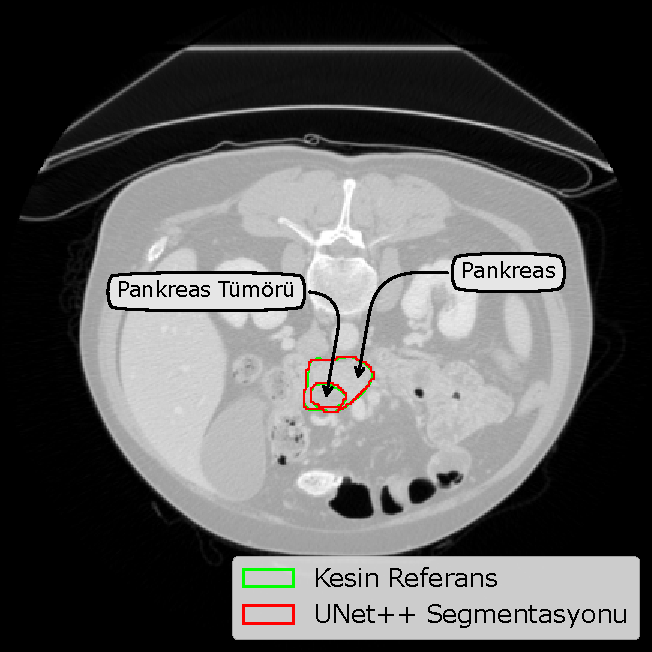
\includegraphics[width=0.3\textwidth]{Bulgular-Irdeleme/Figures/unpp2d1.pdf} & 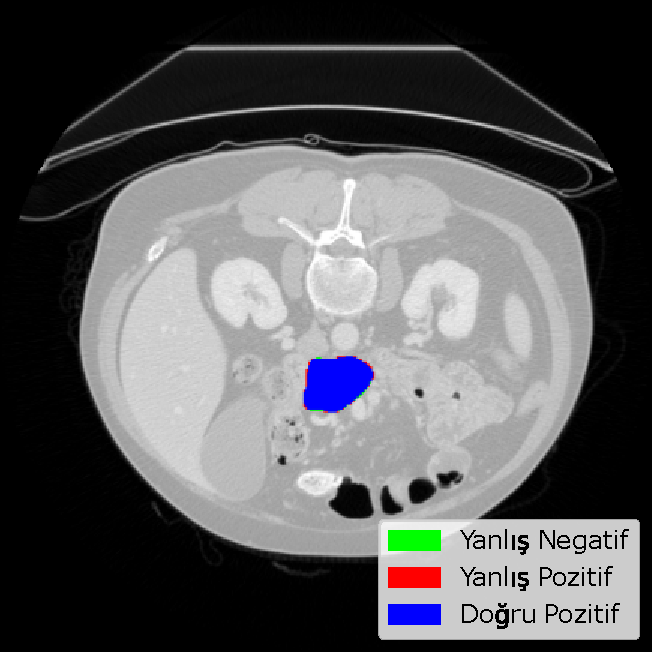
\includegraphics[width=0.3\textwidth]{Bulgular-Irdeleme/Figures/unpp2d2.pdf} & 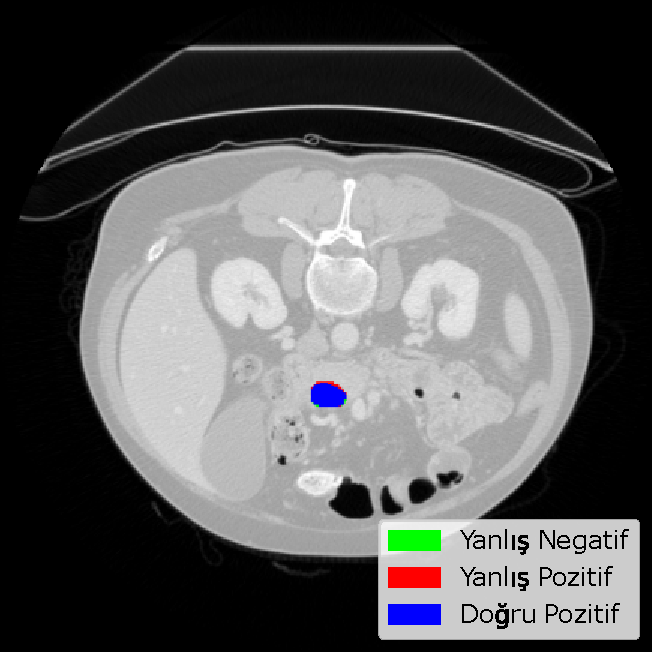
\includegraphics[width=0.3\textwidth]{Bulgular-Irdeleme/Figures/unpp2d3.pdf} \\
				(a) & (b) & (c)\\
				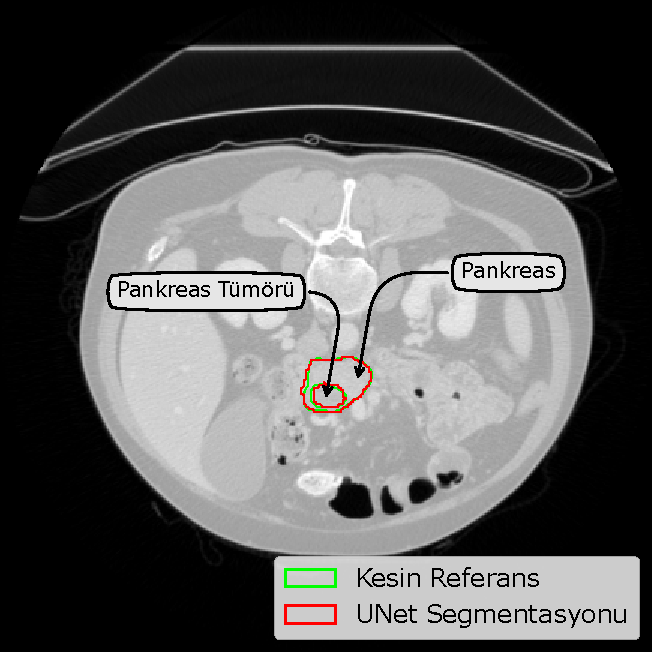
\includegraphics[width=0.3\textwidth]{Bulgular-Irdeleme/Figures/un2d1.pdf} & 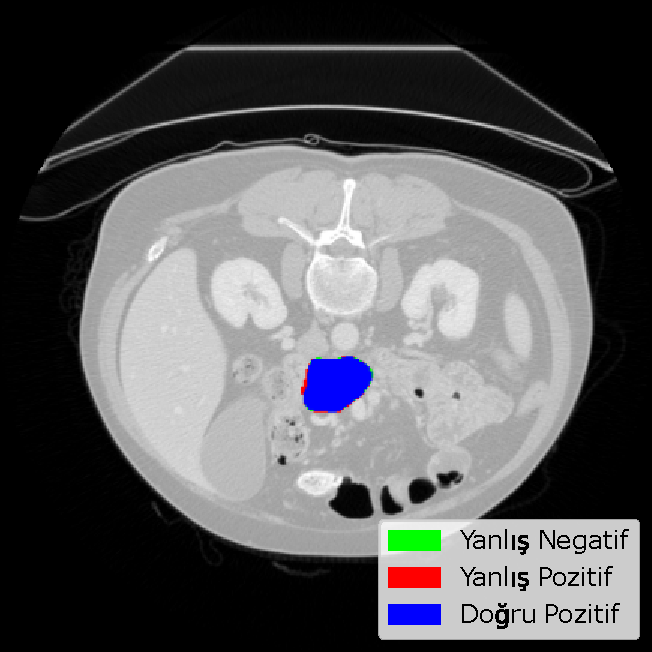
\includegraphics[width=0.3\textwidth]{Bulgular-Irdeleme/Figures/un2d2.pdf} & 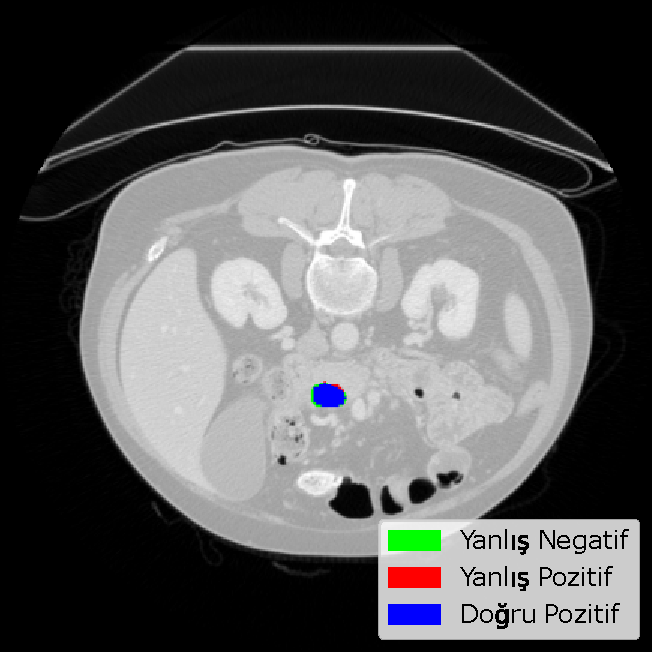
\includegraphics[width=0.3\textwidth]{Bulgular-Irdeleme/Figures/un2d3.pdf} \\
				(d) & (e)  & (f)\\
				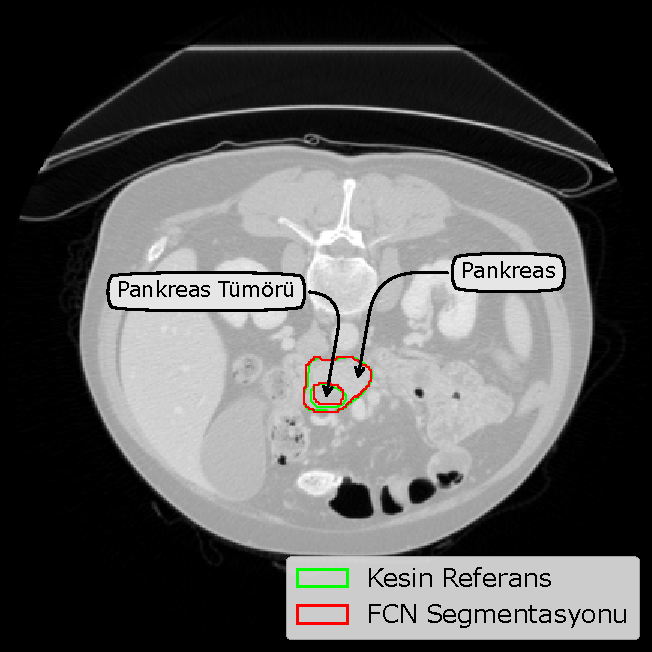
\includegraphics[width=0.3\textwidth]{Bulgular-Irdeleme/Figures/fcn2d1.pdf} & 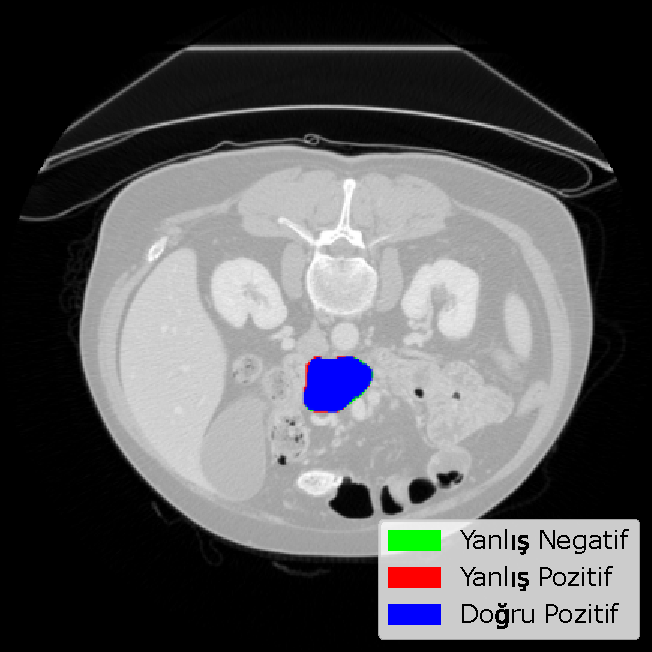
\includegraphics[width=0.3\textwidth]{Bulgular-Irdeleme/Figures/fcn2d2.pdf} & 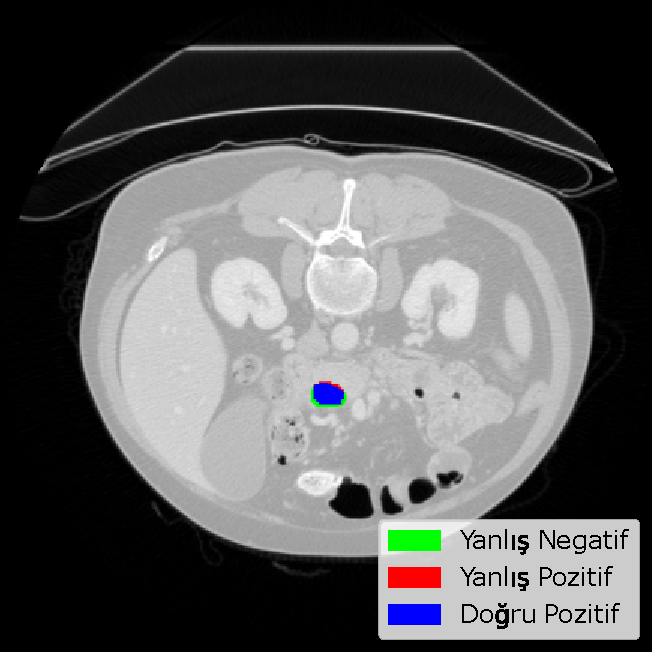
\includegraphics[width=0.3\textwidth]{Bulgular-Irdeleme/Figures/fcn2d3.pdf} \\
				(g) & (h)  & (i)
			\end{tabular}
		}
	\end{center}
\end{figure}

\captionsetup[figure]{margin={1.5cm, 0cm}}
\begin{figure}[h!]
	\begin{center}
		\vspace{0.4cm}
		\captionbox{Radyolog tarafından işaretlenen gerçek referans bölgeleri (a, b, c), Mask R-CNN \& 3B U-Net++ (d, e, f), Mask R-CNN \& 3B U-Net (g, h, i) ve Mask R-CNN \& 3B FCN Oto Kodlayıcı (j, k, l) modelleri kullanılarak elde edilen pankreas ve pankreas tümörü segmentasyon sonuçları
	    \label{fig:results3D}}
		{
			\begin{tabular}{ccc}
				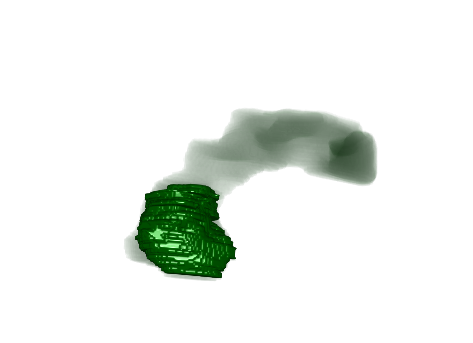
\includegraphics[width=0.3\textwidth]{Bulgular-Irdeleme/Figures/gt3dmix.png} & 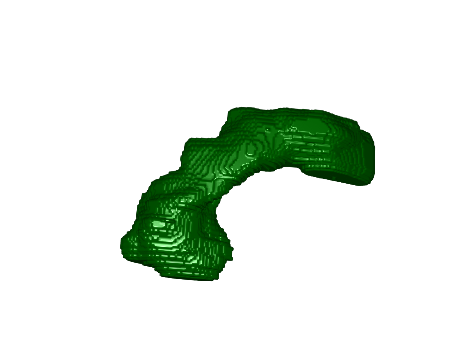
\includegraphics[width=0.3\textwidth]{Bulgular-Irdeleme/Figures/gt3dpan.png} & 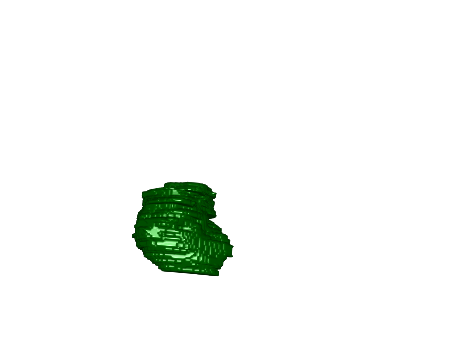
\includegraphics[width=0.3\textwidth]{Bulgular-Irdeleme/Figures/gt3dtum.png} \\
				(a) & (b) & (c) \\
				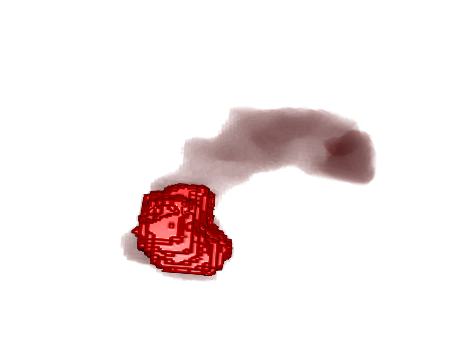
\includegraphics[width=0.3\textwidth]{Bulgular-Irdeleme/Figures/unpp3dmix.png} & 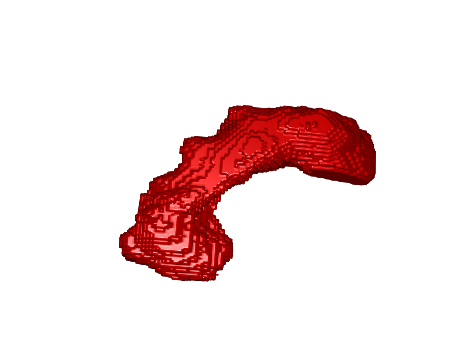
\includegraphics[width=0.3\textwidth]{Bulgular-Irdeleme/Figures/unpp3dpan.png} & 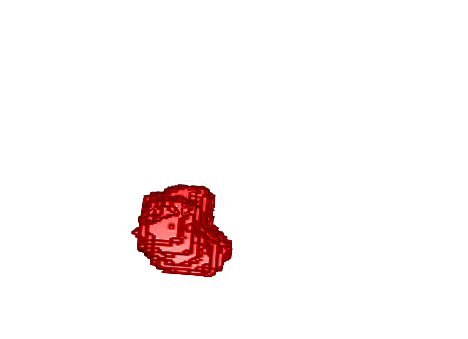
\includegraphics[width=0.3\textwidth]{Bulgular-Irdeleme/Figures/unpp3dtum.png} \\
				(d) & (e) & (f) \\
				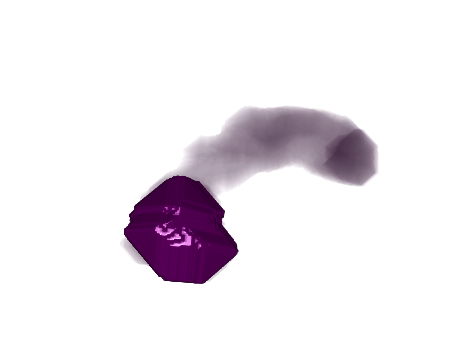
\includegraphics[width=0.3\textwidth]{Bulgular-Irdeleme/Figures/un3dmix.png} & 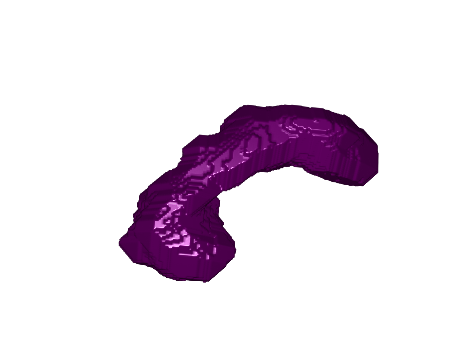
\includegraphics[width=0.3\textwidth]{Bulgular-Irdeleme/Figures/un3dpan.png} & 
\includegraphics[width=0.3\textwidth]{Bulgular-Irdeleme/Figures/un3dtum.png} \\
				(g) & (h) & (i) \\
				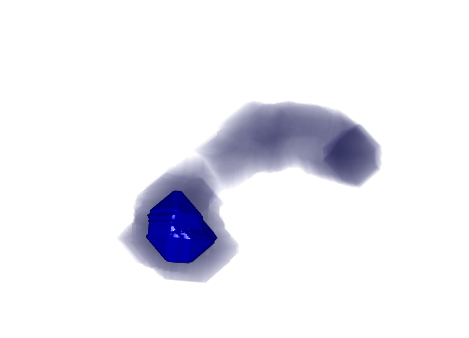
\includegraphics[width=0.3\textwidth]{Bulgular-Irdeleme/Figures/fcn3dmix.png} & 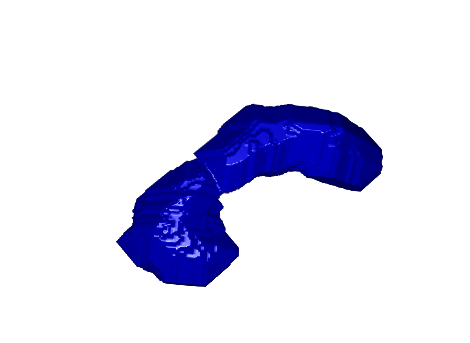
\includegraphics[width=0.3\textwidth]{Bulgular-Irdeleme/Figures/fcn3dpan.png} & 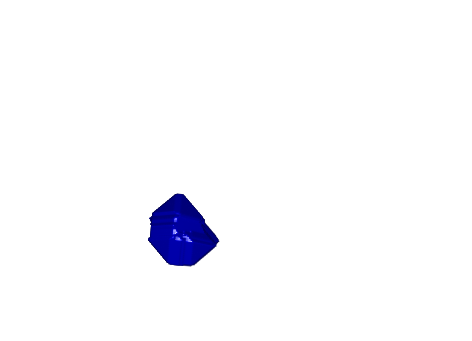
\includegraphics[width=0.3\textwidth]{Bulgular-Irdeleme/Figures/fcn3dtum.png} \\
				(j) & (k) & (l)
			\end{tabular}
		}
	\end{center}
\end{figure}


2B görüntülerde mavi, kırmızı ve yeşil bölgeler sırasıyla DP (doğru segmentlere ayrılmış pankreas bölgesi), YP (geçersiz segmentlere ayrılmış pankreas bölgesi) ve YN'yi (eksik segmentlere ayrılmış pankreas bölgesi) temsil etmektedir. Şekil \ref{fig:results2D}'te her bir satır sırasıyla Mask R-CNN \& 3B U-Net++ (a, b, c), Mask R-CNN \& 3B U-Net (d, e, f) ve Mask R-CNN \& 3B FCN Oto Kodlayıcı (g, h, i) modelleri kullanılarak elde edilen pankreas ve pankreas tümörü segmentasyon sonuçlarını temsil etmektedir. Görsel sonuçlarda, (a,d,g) ile temsil edilen görsellerde farklı segmentasyon algoritmaları için pankreas tümörü ve pankreas segmentasyonu sonuçlarının her ikisi birlikte gösterilmektedir. Görsel sonuçlarda, (b,e,h) ile temsil edilen görsellerde farklı segmentasyon algoritmaları için sadece pankreas segmentasyon sonuçları gösterilmektedir. Son olarak görsel sonuçlarda, (c,f,i) ile temsil edilen görsellerde farklı segmentasyon algoritmaları için sadece pankreas tümör segmentasyonu sonuçları gösterilmektedir.

Şekil \ref{fig:results3D}'da ise radyolog tarafından işaretlenen gerçek referans bölgeleri (a, b, c), Mask R-CNN \& 3B U-Net++ (d, e, f), Mask R-CNN \& 3B U-Net (g, h, i) ve Mask R-CNN \& 3B FCN Oto Kodlayıcı (j, k, l) kullanılarak elde edilen pankreas ve pankreas tümörü segmentasyon sonuçları gösterilmektedir. 3B BT dilimlerinde yeşil, kırmızı, mor ve mavi bölgeler sırasıyla radyolog tarafından manuel olarak işaretlenen, Mask R-CNN \& 3B U-Net++, Mask R-CNN \& 3B U-Net ve Mask R-CNN \& 3B FCN Oto Kodlayıcı ile segmentlere ayrılmış pankreas ve pankreas tümörü bölgelerini temsil etmektedir. Görsel sonuçlarda (a,d,g,j) ile temsil edilen görsellerde 3B pankreas ve pankreas tümörü her ikisi birlikte gösterilmektedir. Görsel sonuçlarda (b,e,h,k) ile temsil edilen görsellerde 3B pankreas segmentasyon sonucu gösterilmektedir. Son olarak, görsel sonuçlarda (c,f,i,l) ile temsil edilen görsellerde 3B pankreas segmentasyon sonucu gösterilmektedir.  Şekil \ref{fig:results2D} ve \ref{fig:results3D}'daki 2B ve 3B görsel sonuçlardan radyolog tarafından manuel olarak işaretlenen bölgelere en benzer sonuçların Mask R-CNN \& 3B U-Net++ ile elde edildiği çıkarılmaktadır. 

